\documentclass[12pt,letterpaper]{article}

%%%%%%%%%
%   Packages	 %
%%%%%%%%%

\setlength\parindent{0pt} % para desindentar los párrafos
\setlength{\parskip}{1em} % espacio entre los párrafos
\renewcommand{\baselinestretch}{1.5} % espacio entre líneas
\usepackage[letterpaper, margin=0.8in]{geometry}

% Floats
\usepackage{graphicx}
\usepackage{float}
\restylefloat{figure}
\usepackage{subfigure}
\usepackage{subfig}
\usepackage{color}

% Math packages
\usepackage{amsmath}
\usepackage{amsfonts}
\usepackage{amssymb}

% To make pretty tables
\usepackage{booktabs}
\usepackage{multirow}
\usepackage{array}

% To avoid underfull errors in the bibliography
\usepackage{etoolbox}
\apptocmd{\sloppy}{\hbadness 10000\relax}{}{}

% To make cites and references
\usepackage[hidelinks,pdfusetitle,pdfdisplaydoctitle]{hyperref}
\usepackage[notocbib]{apacite} 
\usepackage{doi}
\renewcommand{\doitext}{}

% Español y acentos
\usepackage[utf8]{inputenc}

% Ajustar tablas
\usepackage{adjustbox}
\usepackage{dcolumn}

% Horizontal
\usepackage{lscape}
\usepackage{rotating}

%Listas
\usepackage[shortlabels]{enumitem}
\setlist[enumerate, 1]{1\textsuperscript{o}}

%opening
\title{Preferencias redistributivas en contextos desiguales: Cambios en América Latina entre 2008 y 2014}
\author{Gonzalo Franetovic\\ Juan Carlos Castillo}

\begin{document}

\maketitle

\begin{abstract}

En una región en vías de desarrollo y altamente desigual como América Latina, resulta trascendental la comprensión de los determinantes que afectan en el acuerdo de las personas con la redistribución de recursos desde el estado. La popular hipótesis del votante mediano y las teorías centradas en el autointerés han establecido continuamente un vínculo negativo entre el ingreso que tienen las personas y su apoyo hacia la disminución de desigualdades vía redistribución. A pesar de ello, la evidencia es escasa y a veces contradictoria, mientras que su testeo en Latinoamérica resulta casi inexistente. Utilizando datos de la Encuesta LAPOP entre los años 2008 y 2014, esta investigación se centra en la hipótesis del autointerés, pero tomando en cuenta la influencia del nivel de desigualdad de los países así como también el nivel de desarrollo económico. Para ello, se emplean modelos híbridos de regresión multinivel, sobre 4 períodos de tiempo entre 2008 y 2014 y 18 naciones, controlando por características relevantes tanto de los países como de los individuos. Los resultados dan cuenta de escasas diferencias entre quintiles económicos en preferencias redistributivas, por lo que las diferencias de ingreso no lograrían constituirse como un determinante esencial sobre las preferencias redistributivas de la población latinoamericana de manera general, aunque si en aquellas con mayor nivel de desarrollo económico. A la luz de los resultados, se establecen comparaciones con los hallazgos de investigaciones previas en países desarrollados, discutiéndose la aplicación de teorías racionalistas en materia de justicia y solidaridad social dentro de la región.

\end{abstract}

\newpage

\section{INTRODUCCIÓN \label{sec:sec1}}

América Latina es una región marcada por la desigualdad y la presencia de países sub-desarrollados o en vías de desarrollo. Con todo, son innegables los progresos evidenciados por gran parte de los países en las últimas décadas en materia distributiva (Lustig, Lopez-Calva, \& Ortiz-Juarez, 2013) y de superación de la pobreza (Dayton-Johnson, 2013). Sin embargo, un gran cúmulo de evidencia concluye que nuestra región se sitúa como la más desigual a nivel mundial (Bird, 2013; CEPAL, 2015) y, lo que es más grave, que conserva dicha posición sostenidadmente desde mediados del siglo pasado (Mann \& Riley, 2007). Ante este contexto, resulta trascendental preguntarse por los factores que afectan la redistribución de los ingresos.\\

Como comúnmente se ha reconocido, la redistribución manifiesta una tremenda importancia al constituirse como una de las mayores herramientas que posee una sociedad para luchar contra la pobreza y la desigualdad, los principales retos que posee nuestra región (Hoffman \& Centeno, 2003). Como es de suponer, en aquellas sociedades donde existe una mayor demanda por la acción redistributiva del Estado, existen también mayores chances de que esta última se materialice vía elección de representantes que favorezcan la redistribución mediante políticas públicas. Por lo mismo, identificar el grado de acuerdo de las personas con la redistribución y comprender los principales determinantes que lo explican resulta un ejercicio de gran importancia, más aún en contextos de alta pobreza y desigualdad como es América Latina. En este marco el presente estudio se orienta por la siguiente pregunta: \textbf{¿cómo son y cómo cambian las preferencias redistributivas de las personas en sociedades con alta desigualdad económica y en vías de desarrollo?}. Si bien en general se asume que las personas de mayores ingresos se verán más reacias a la acción redistributiva del Estado por cuestiones de autointerés, la mayor parte de las investigaciones hasta ahora se han implementado en contextos comparativamente igualitarios, por lo que se abre la pregunta de si la desigualdad sería un elemento que potenciaría la presión por la redistribución y de esta manera aminoraría las diferencias entre individuos de distintos niveles socioeconómicos en sus preferencias redistributivas. Además, la evidencia a la fecha presta escasa atención al cambio de las preferencias en el tiempo y cómo las variaciones en niveles de desigualdad podrían también repercutir en el apoyo a la redistribución. \\

La falta de estudios sobre preferencias redistributivas en contextos desiguales y también sobre su cambio se debe principalmente a la dificultad de contar con datos específicos que contengan estas variables. Sin embargo, la encuesta del Latin American Public Opinion Project (LAPOP) entrega la oportunidad de analizar en un horizonte de tiempo de seis años (2008-2014) las preferencias distributivas en 18 países de América Latina, lo cual no tiene precedentes en la región. Además, el análisis y modelamiento de cambio con datos cross-seccionales ha sido un tema que se ha expandido solo recientemente con la estimación de modelos multinivel para datos repetidos cross-seccionales (Schmidt-Catran, 2016) (o más genéricamente, modelos híbridos) y que hasta el momento no han sido vista aplicados a nuestra región ni tampoco a nivel internacional en el ámbito de preferencias, representando por tanto una doble oportunidad de innovación.\\

El estudio se estructura en cinco principales secciones. Primero, se discute evidencia respecto a determinantes individuales y nacionales en preferencias redistributivas, centrándose en el enfoque de autointerés y las críticas que sobre éste se han establecido. En la segunda sección, se describe la metodología utilizada, incluyendo detalles respecto a la muestra, las variables y los modelos híbridos de regresión multinivel utilizados. En tercer lugar, se exponen los resultados, divididos en dos sub-secciones: análisis descriptivo, identificando tendencias nacionales y temporales del acuerdo con la redistribución; y estimación multinivel, presentando los resultados de los modelos estadísticos y la forma en que éstos comprueban o refutan las hipótesis planteadas. La cuarta sección discute con la literatura los resultados evidenciados y la última sección da cuenta de las principales conclusiones que surgen de la presente investigación, así como sus limitaciones y las futuras lineas de estudio a partir de los hallazgos. 

\newpage

\section{Redistribución y desigualdad \label{sec:sec2}}

Con el acrecentamiento de las desigualdades, el alza en la concentración de riquezas y la crisis de los estados de bienestar a lo largo de una gran gama de países, las preferencias por redistribución se han constituido en un tópico que ha concentrado cada vez más interés académico, insertándose en una discusión donde comparte terreno con actitudes hacia el estado de bienestar, formas de solidaridad social, percepción y legitimación de desigualdades, entre otros. Dado que el presente estudio surge de la comprobada premisa respecto a que las actitudes hacia las políticas públicas pueden ser comprendidas por explicaciones a diferentes niveles (Alesina \& Giuliano, 2009), la revisión de literatura se estructurará en dos secciones: en primer lugar, respecto a los determinantes de carácter individual (Alesina \& Giuliano, 2009; Franko, Tolbert, \& Witko, 2013a; McCall, 2013) y, en segundo, aquellos a nivel país (Edlund, 1999; Isaksson \& Lindskog, 2009; Kenworthy \& McCall, 2007).

\subsection{Factores individuales de las preferencias redistributivas \label{sec:sec21}}

\subsubsection{Autointerés, ingreso y posición objetiva \label{sec:sec211}}

Si existe una certeza al interior del estudio de preferencias redistributivas, es que la gran mayoría le otorga a la teoría de votante mediano un rol pionero y fundamental en la discusión (Alesina \& Giuliano, 2009; Berens, 2015a; A. M. J. Castillo \& Sáez Lozano, 2010; J. C. Castillo, Palacios, Joignant, \& Tham, 2015; Dhami \& al-Nowaihi, 2010; Keller, Medgyesi, \& Tóth, 2010; Luebker, 2004; McCall, 2013). En su clásico modelo, Meltzer \& Richard (1981), basándose en Romer (1975), establecen que en tanto mayor sea la desigualdad en los países, mayor tenderá a ser el apoyo al gasto social por parte de los votantes, redundando en un incremento en la redistribución efectiva de riquezas entre ricos y pobres. En la medida que sea menos equitativa la distribución de recursos, el votante de ingreso mediano será más pobre que el votante de ingreso promedio, por lo cual la mayoría de los individuos poseerán incentivos para votar a favor de la redistribución; cuestión que, en un contexto democrático y de elecciones abiertas, culminará con una efectiva mayor redistribución de recursos al interior de una sociedad. Así, mediante esta relación entre desigualdad y redistribución, las sociedades mantendrían una suerte de autorregulación distributiva\footnote{Como bien sintetiza Schmidt-Catran (2016), este teorema basa su línea argumental en un mecanismo constituido por variados supuestos. En países con una distribución de ingresos con mediana menor a la media -en el presente, la mayoría sino la totalidad de las sociedades contemporáneas- se espera: (i) que el votante mediano exija redistribución y esta demanda sea mayor a medida que los ingresos sean menores; (ii) que esta petición por redistribución posteriormente se exprese de forma directa en las votaciones y preferencias políticas; y (iii) que los partidos políticos respondan consecuentemente ante este requerimiento, en su necesidad por mantener apoyo de la población. Dadas las especificidades del presente estudio, interesa la primera fase de este teorema: aquella que vincula el ingreso de los sujetos con su apoyo por el gasto fiscal y la reducción de desigualdades.}.\\

A partir de estos postulados, se erige una de las dos principales aproximaciones que han tendido a explicar el grado de apoyo de los sujetos hacia la redistribución desde un plano individual. Conocida bajo el rótulo de “enfoque de autointerés”, esta perspectiva supone una directa relación entre la posición socioeconómica que ocupa el sujeto al interior de la estructura social y sus interpretaciones y disposiciones en materia de justicia distributiva. Se sostiene, entonces, que la posición albergada por los sujetos determina una diferente exposición ante el riesgo -de caer en una situación económicamente no deseada- y que este último sería el encargado de generar diferentes patrones de autointerés (Wegener \& Liebig, 2000). Así, esta perspectiva avala que la posición relativa ante el riesgo, experimentada diferenciadamente por los sujetos, sería un condicionante esencial de la importancia que se le atribuye a la redistribución (Barth, Finseraas, \& Moene, 2015; Rehm, Hacker, \& Schlesinger, 2012).\\

Variados son los factores que la literatura identifica respecto a las discrepancias de riesgo experimentado. Determinantes como el estatus -en términos de nivel educacional u ocupacional- o la clase social de pertenencia –a nivel de posición en la estructura productiva- se sitúan como determinantes del autointerés expresado por las personas, así como la condición laboral (Gijsberts, 2002). Sin embargo, el determinante más comúnmente analizado es el ingreso. En adición a lo establecido por Meltzer \& Richard (1981), Franko, Tolbert, \& Witko (2013) afirman que la pertenencia a un estrato bajo se asocia sostenidamente a mayores tendencias por apoyar un aumento en la redistribución, que significa un incremento de carga tributaria a los más ricos. Esta relación negativa entre ingreso y redistribución ha sido evidenciada también por Bernasconi (2006), Iversen (2005), Jæger (2005, 2006) y Finseraas (2009), todos avalando la significativa tendencia a la baja que manifiesta el acuerdo con la redistribución a medida que el ingreso de las personas aumenta. La explicación en esta relación ampliamente apoyada encuentra sustento en lo que Szirmai (1986) entiende bajo la idea de “deprivación absoluta”: las personas con mayores niveles de ingreso legitimarán una mayor desigualdad porque una disminución de brechas tenderá a desfavorecerlos. Del mismo modo, personas con bajos ingresos preferirán una menor desigualdad, en tanto se verán beneficiados respecto a su condición actual; cuestión que, en última instancia, se vincula con el convencimiento de cada individuo por considerar o no la redistribución como una acción deseable.


\subsubsection{Crítica al autointerés: El homo-sociologicus \label{sec:sec212}}

A pesar del apoyo que encuentra la teoría del autointerés en el sentido común y en una serie de investigaciones, también existen propuestas y evidencias que se distancian de las meras razones instrumentales del homo-economicus, señalando como contrapartida a un homo-sociologicus que contempla cultura, valores y creencias que van más allá del interés personal (Feldman \& Zaller, 1992). Por ello, cuestiones como la identificación política (Castillo, Madero-Cabib, \& Salamovich, 2013) y en el sistema tributario (Alm \& Torgler, 2006), así como la religión (Scheve \& Stasavage, 2006), son elementos que han tendido a ser relacionados con la configuración del apoyo por redistribución. De la misma forma ocurre con la confianza en el sistema político: se asume que, mientras las personas consideren que las instituciones gubernamentales operan basadas en principios como la eficacia y la probidad, es más probable que apoyen políticas de bienestar (Kumlin, 2004), como la redistribución de recursos y otras.\\

Particularmente con respecto a América Latina, la acción del autointerés en la conformación de preferencias por redistribución también ha sido puesta en tela de juicio. Berens (2015) ha centrado su análisis en las características de la región y las diferencias entre trabajadores formales e informales. Según el enfoque de autointerés, las personas con empleo irregular tenderían a poseer una mayor preferencia por la redistribución, en tanto su actividad económica, al estar al margen del sistema formal de trabajo, no conlleva la aplicación de impuestos asociados. Sin embargo, el análisis de Berens (2015) revela que justamente esta relación operaría a la inversa, siendo el interés más influyente sobre los trabajadores formales que informales al interior de la región, contrario a lo evidenciado por Schmidt-Catran (2016) donde en países desarrollados la población desempleada se configura como el estrato laboral que más demanda redistribución. Al igual como plantean Dion \& Birchfield (2010), la concepción de sujeto racional que guía los teoremas de votante mediano y el enfoque de autointerés no se manifestaría de la misma forma a lo largo del planeta. Sin embargo, y dado que el tema de las preferencias redistributivas ha sido escasamente estudiado en la región, nuestro planteamiento inicial explora la perspectiva más bien tradicional del autointerés, de lo que se desprende la primera hipótesis del estudio:

\textit{H1: El ingreso de las personas estará negativamente relacionado con el acuerdo individual por redistribución}

\subsection{Factores contextuales de las preferencias redistributivas \label{sec:sec22}}

En adición a las propias características que definen a los sujetos a nivel individual, se ha observado que las preferencias y actitudes en materia distributiva se ven altamente influidas por elementos del contexto en el cual estas personas viven (Wegener \& Liebig, 1995; Forsé \& Parodi, 2007). Dada su particular importancia en materia de acuerdo con la disminución de brechas económicas entre la población, se abordará la discusión respecto a dos principales determinantes a nivel nacional: la desigualdad y el desarrollo económico\footnote{Si bien ha sido comúnmente abordada la discusión respecto a los Estados de Bienestar (Esping-Andersen, 1990a, 1990b) y su influencia en las concepciones de las personas ante la desigualdad y la redistribución en países desarrollados (Esping-Andersen \& Myles, 2011; Svallfors, 1997), la limitada presencia de regímenes de bienestar consolidados en la región (Haggard \& Kaufman, 2008; Marcel \& Rivera, 2008), obliga a redirigir la discusión centrándose en los determinantes que podrían tener injerencia, ser comprobados o refutados en el contexto a analizar. Aún así, en adelante se incluye una tipología exploratoria de regímenes de bienestar latinoamericanos (Martínez Franzoni, 2008) en los modelos estadísticos, sin evidenciar mayores influencias.}.

\subsubsection{Desigualdad económica \label{sec:sec221}}

Tal como señalabamos anteriormente para el caso de los factores individuales, según Meltzer \& Richard (1981) en tanto mayor sea la desigualdad en los países, mayor será la probabilidad de que los individuos manifiesten un acuerdo con la redistribución. Esta relación puede también considerarse en un sentido dinámico y por tanto debiese aplicar tanto "entre" los países como "dentro de" los países, en la medida que cualquier aumento en la desigualdad de un país producirá, asimismo un movimiento en la relación votante medio - votante mediano, haciendo previsible una demanda mayor aún por redistribución a lo largo de la población.\\

Sin embargo, la evidencia empírica nos muestra que esta relación resulta más compleja de lo que parece, evidenciándose cómo en muchos casos sociedades con mayor desigualdad incluso presentan una mayor tolerancia ante esta última (Castillo, 2010; Sachweh \& Olafsdottir, 2012). Con ello, un buen número de estudios ha tendido a problematizar la aplicabilidad que posee la teoría de votante mediano desde un enfoque transversal -“entre” países- (Alesina \& Glaeser, 2004; Kenworthy \& Pontusson, 2005), como longitudinal -"dentro de" países. Utilizando información para ocho naciones entre 1980 y 1990, Kenworthy \& McCall (2007) concluyen que las variaciones en la desigualdad “dentro de” los países no se asociarían a un consecuente cambio en la generosidad de las políticas redistributivas. Mismo caso con Schmidt-Catran (2016) en países europeos, quien encuentra sustento para la teoría de votante mediano a nivel transversal pero no longitudinal.\\

Además, autores contemporáneos han visto cómo la desigualdad de ingresos (Atkinson, Piketty, \& Saez, 2011; E. Huber \& Stephens, 2001), las divisiones entre incluidos y excluidos (Rueda, 2008), y el desempleo (Rehm, 2011) se han vuelto fenómenos mucho más frecuentes, sin una conducente reducción de desigualdades en países desarrollados. A pesar de ello, los países latinoamericanos parecen manifestar una tendencia diferente los últimos años, donde se ha visto una expansión de sus políticas sociales favorables a los más pobres (Garay, 2010; Mares \& Carnes, 2009). Todo esto anticipa posibles falencias por parte del modelo clásico de votante mediano a nivel macro para el caso latinoamericano, pero nuevamente argumentando desde una perspectiva más tradicional y racional, nuestra segunda hipótesis propone que:\\

\textit{H2a (entre): Los niveles de desigualdad económica de los países estarán positivamente relacionados con el apoyo a la redistribución.}

\textit{H2b (dentro): Los cambios en la desigualdad económica de los países estarán positivamente relacionados con el apoyo a la redistribución.}\\

Junto con el posible efecto directo de la desigualdad en las preferencias por la redistribución, es dable pensar que la desigualdad económica de los países podría tener además un efecto moderador, afectando la forma en que variadas características individuales se relacionan con la demanda por redistribución. Autores como Lupu \& Pontusson (2011) y Luttig (2013), plantean que la estructura de la desigualdad guarda especial relevancia. Para ellos, a medida que el estrato económico medio (percentil 50) se ubique más próximo en ingresos al estrato bajo (percentil 10), generará una mayor afinidad social con las clases desposeídas. Esta acción, comprendida como altruismo parroquial según Fowler \& Kam (2007), se distingue del altruismo generalizado en tanto se basa en una identificación social compartida con grupos particulares de la sociedad (Goette, Huffman, \& Meier, 2006). Así, en sociedades más desiguales existiría una menor diferencia en las preferencias redistributivas a lo largo de los diferentes estratos de ingreso, por la constitución de un grupo más reducido de privilegiados y la consecuente emergencia de sentimientos de solidaridad y afinidad mayormente compartidos a lo largo de la población no beneficiada. Por lo tanto, basados en los conceptos de afinidad social y altruismo parroquial, la tercera hipótesis del estudio es:

\textit{H3: En los países más desiguales habrá un apoyo más transversal a la redistribución a través de los distintos niveles de ingreso individual.}

\subsubsection{Desarrollo económico \label{sec:sub222}}

Un segundo factor a nivel estructural que la literatura ha abordado en términos de bienestar y justicia distributiva es el desarrollo económico, comúnmente medido a través del Producto Interno Bruto per cápita de los países. Entre la bibliografía más clásica, el nexo entre crecimiento y distribución de recursos ha estado marcado por la conocida curva propuesta por Kuznets (1955): a medida que los países se desarrollan, su desigualdad también se incrementa, hasta un punto donde el crecimiento comienza a retornar distribuciones de ingreso cada vez más equitativas\footnote{A pesar de ser formulada en sus orígenes para naciones industrializadas, este teorema ha sido aplicado a una vasta gama de contextos (Alvaredo, 2007; Atkinson et al., 2011; Williamson, 2015)}. Sin embargo, en materia de preferencias distributivas, comúnmente el desarrollo económico ha tendido a ser considerado como una variable de control (Rudra, 2002; Schmidt-Catran, 2016; Schröder, 2017), siendo escasos los intentos por establecer una relación directa y explicativa entre la riqueza de los países y las actitudes hacia la redistribución de recursos de sus ciudadanos\footnote{Entre esos pocos, Finseraas (2009), dentro de una muestra de 22 naciones europeas, establece que aquellas más desarrolladas presentan en promedio un menor apoyo hacia la redistribución, pero su efecto no consigue constituirse como estadísticamente significativo.}\\

A pesar de ello, existe un mecanismo causal que no vincularía al desarrollo económico de forma directa sobre las preferencias redistributivas, pero sí albergaría alto poder explicativo al generar influencia sobre las configuraciones valóricas de los sujetos: la teoría de cambio cultural. Según Inglehart (1977), la modernización conlleva la emergencia de valores postmaterialistas al interior de las sociedades. El crecer en espacios de seguridades existenciales y necesidades básicas cubiertas, influirá en la configuración de sujetos identificados menos con preocupaciones económicas y más con preferencias liberales, autónomas y atentos a necesidades ulteriores de realización personal (Inglehart, 2008), las cuales se han visto vinculadas a las visiones de solidaridad y estado de bienestar que tienen las personas (Gelissen, 2000), estrechamente relacionadas a las preferencias por redistribución.\\

A partir de ello, se extraen las siguientes hipótesis de la investigación:

\textit{H4a: Los niveles de desarrollo económico de los países estarán positivamente relacionados con el apoyo a la redistribución.}

\textit{H4b: Los cambios en el desarrollo económico de los países estarán positivamente relacionados con el apoyo a la redistribución.}\\

\begin{figure}[t]
	\begin{center}
		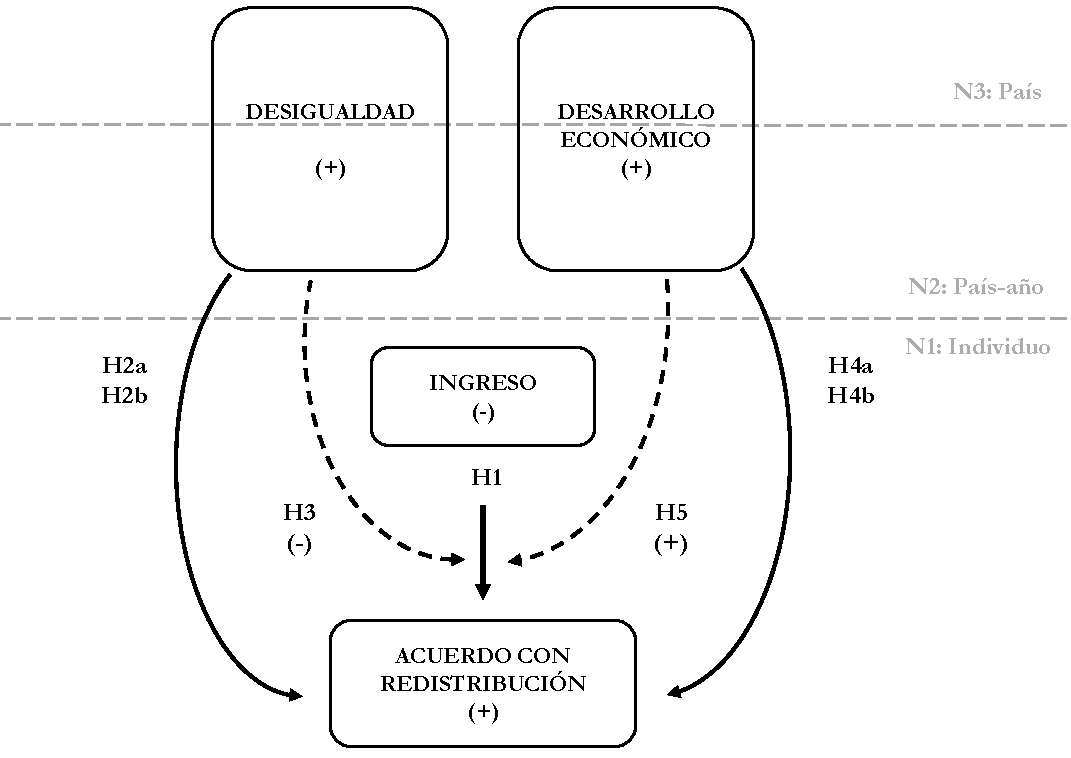
\includegraphics[width=1\textwidth]{Hipotesis.pdf}
		\caption[Diagrama de hipótesis]{Diagrama de hipótesis}
		\label{fig:hip}
	\end{center}
\end{figure}

Al igual como fue planteado el efecto moderador de la desigualdad, se ha visto cómo el desarrollo económico es capaz de modificar el efecto que ejercen ciertas características de las personas -como el ingreso- sobre sus propias preferencias por redistribución. Según Reenock, Bernhard, \& Sobek (2007), la emergencia de reacciones extremas según estrato socioeconómico se dará exclusivamente en ambientes caracterizados por una “distribución socioeconómica regresiva”, donde convivan un acentuado desarrollo económico y carencias elementales. Coincidentemente, Bowles \& Gintis (2000) establecen que el apoyo al estado de bienestar tiende a estar ligado a obligaciones morales básicas con los otros, en pos de asegurar la provisión de estándares mínimos de bienestar, primando un Homo sociologicus por sobre el clásico Homo economicus de las concepciones economicistas clásicas. Por ello, en sociedades con menores niveles de desarrollo económico, donde la garantía y cobertura de dichas necesidades básicas se encuentra menos asegurada, el autointerés operaría en menor medida sobre la configuración de las preferencias de las personas, redundando en menores diferencias hacia la redistribución a través de los estratos de ingreso (Dion \& Birchfield, 2010). En concreto, una persona de bajos ingresos en un país de mayor desarrollo económico exigiría comparativamente más redistribución que alguien de bajos ingresos en un país de menor desarrollo económico. Por lo tanto, es posible plantear que: 

\textit{H5: En los países con mayor desarrollo económico, la relación entre el ingreso y el apoyo a la redistribución será más fuerte que en países menos desarrollados.}\\

La Figura \ref{fig:hip} resume las hipótesis planteadas. Se diferencia el nivel individual, contextual (país) y también temporal (país-año), dado que cada país posee cuatro mediciones en el tiempo. Además de los efectos directos en redistribución, la línea punteada simboliza el efecto moderador de las variables contextuales en la relación entre ingreso y acuerdo con la redistribución. 

\section{METODOLOGÍA \label{sec:sec3}}

\subsection{Datos \label{sec:sec31}}

El presente estudio busca caracterizar a lo largo del tiempo y determinar el efecto de factores individuales y nacionales sobre el acuerdo individual con la redistribución de recursos al interior de América Latina. Para ello, se utiliza información de 18 países de la región, para los años 2008, 2010, 2012 y 2014. Los datos a nivel individual provienen del Proyecto de Opinión Pública de América Latina (LAPOP) para las olas correspondientes a los mencionados 4 años. La información a nivel país surge de la Base de Datos CEPALSTAT de la Comisión Económica para América Latina y el Caribe (CEPAL), que aúna información proveniente de las principales encuestas socioeconómicas aplicadas a hogares por parte de los mismos Estados latinoamericanos. Así, el estudio contempla una muestra estratificada en 3 niveles, componiéndose de: 82.866 individuos\footnote{Observaciones que poseen valores válidos para la totalidad de variables de interés a nivel individual.} (nivel 1), anidados en 72 unidades país-año (nivel 2), anidados en 18 países\footnote{Se excluye únicamente a Cuba y Puerto Rico, dada su escasez de información económica a nivel país.} (nivel 3).

\subsection{Variables \label{sec:sec32}}

\subsubsection{Variables individuales \label{sec:sec321}}

La variable dependiente del estudio es el acuerdo individual con la redistribución, que nace de la pregunta: "El Estado (gentilicio) debe implementar políticas firmes para reducir la desigualdad de ingresos entre ricos y pobres. ¿Hasta qué punto está de acuerdo o en desacuerdo con esta frase?”. Esta variable oscila entre los puntajes 1 (“muy en desacuerdo”) y 7 (“muy de acuerdo”).\\

El ingreso mensual del hogar se establece como la principal variable independiente. Para las olas 2008 y 2010 de LAPOP, el ingreso mensual del hogar se encuentra dividido en diez intervalos, ajustados a la moneda nacional de cada país. Sin embargo, para 2012 y 2014, estos intervalos son dieciséis. Para solucionar este inconveniente y poder medir el efecto que tiene la ubicación económica de los sujetos respecto a su contexto -mismo espacio y tiempo- sobre sus preferencias por redistribución, se utilizó recodificación automática\footnote{En países-año donde la distribución de la variable original de ingreso se encontraba sesgada, se generó recodificación manual para asegurarse la existencia de quintiles de ingreso, equitativamente repartidos.}, generándose quintiles de ingreso, para cada país-año. Así, el ingreso se constituye como una variable continua, que oscila entre 1 (quintil más pobre) y 5 (quintil más rico).\\

Por otro lado, hay variables a nivel individual que son reconocidas por la literatura como influyentes a la hora de estimar las preferencias por redistribución (A. M. J. Castillo \& Sáez Lozano, 2010). Como sostienen Brady y Finnigan (2014, p. 21) "bastante consistentemente, los encuestados viejos, mujeres, no casados, menos educados, desempleados y de menor ingreso tienden a apoyar más políticas sociales". Dicho lo anterior, se controlará por las siguientes variables: (i) \textit{sexo} (mujer = 0; hombre = 1); (ii) \textit{edad} medida en años; (iii) \textit{estado civil} (no casados = 0; casados o convivientes = 1); (iv) \textit{ideología política}, oscilando entre 1 (derecha) y 10 (izquierda); (v)  \textit{situación laboral}: en categorías "no pertenecientes a la fuerza laboral", "desempleados" y "empleados"; (vi) \textit{educación}, en categorías de "educación primaria completa o menos", "educación secundaria completa o menos" y "educación terciaria incompleta o completa". (vii) \textit{zona de residencia} (rural = 0; urbano = 1). Asimismo, se controla por la (viii) \textit{confianza en el sistema} que, en la misma linea de Brandt (2013) y Cichocka et al. (2017), corresponde al promedio de la confianza expresada por las personas respecto a variadas instituciones, en este caso, seis: el Ejecutivo, el Congreso Nacional, el sistema judicial, los partidos políticos, las Fuerzas Armadas y la policía nacional; oscilando entre los valores 1 y 7. 

\subsubsection{Variables nacionales \label{sec:sec322}}

La desigualdad económica es medida de la misma forma que los principales estudios en la materia lo han hecho, mediante el coeficiente Gini, que oscila entre los valores 0 (escenario de completa igualdad, donde todos los individuos poseen mismos ingresos) y 1 (completa desigualdad, donde un individuo posee la totalidad de los ingresos)\footnote{Para mejorar su interpretación, la variable fue multiplicada por un factor de 100, de forma que varíe entre 0 y 100}. El desarrollo económico corresponde al Producto Interno Bruto (PIB) anual por habitante por objeto del gasto a precios constantes (de 2010) en miles de dólares. Ambos indicadores se encuentran disponibles para cada unidad país-año\footnote{Para reducidas unidades país-año el coeficiente Gini no contaba con disponibilidad de información. En dichos casos de se optó por la siguiente estrategia: (i) utilizar la información para el año anterior al faltante; (ii) en caso de no poder realizarse el procedimiento (i), utilizar la información del año siguiente al faltante; (iii) en caso de no poder realizarse los procedimientos (i) o (ii), se asigna el resultado de la interpolación lineal entre el dato del año previo más próximo con datos existentes y el dato del año posterior más próximo con datos existentes.}. \\

Otra variable de control corresponde al régimen de bienestar\footnote{También se pretendió controlar por variables como el gasto social de los países y la tasa de informalidad laboral, ambas variables que la literatura reconoce como influyentes. Sin embargo, la gran cantidad de casos perdidos involucraba una pérdida no menor de países que ponía en compromiso el propósito de establecer un estudio para la región en su completa diversidad.}, que surge del análisis de clústers realizado por Martínez Franzoni (2008)  justamente para los 18 países estudiados. En función de aspectos como el mercado laboral, las familias y las políticas públicas de cada país, la autora avala la existencia de 3 grandes tipos de regímenes en América Latina: (i) productivistas: Argentina y Chile; (ii) proteccionistas: Brasil, Costa Rica, Panamá y México; e (iii) informales familiares: Ecuador, El Salvador, Guatemala, Colombia, Venezuela, Perú, República Dominicana, Honduras, Nicaragua, Bolivia y Paraguay.

\begin{table}[t] \centering 
	\caption{Estadísticos descriptivos} 
	\label{tab1}
    \renewcommand{\arraystretch}{0.7}
	\begin{tabular}{@{\extracolsep{5pt}}lccccc} 
		\\[-1.8ex]\hline 
		\hline \\[-1.8ex] 
		Estadístico & \multicolumn{1}{c}{N} & \multicolumn{1}{c}{Media / \%} & \multicolumn{1}{c}{Desv.Est.} & \multicolumn{1}{c}{Min} & \multicolumn{1}{c}{Max} \\ 
		\hline \\[-1.8ex] 
		Ac. redistribución & 82.866 & 5,671 & 1,604 & 1 & 7 \\ 
		Ingreso & 82.866 & 2,859 & 1,411 & 1 & 5 \\ 
		Edad & 82.866 & 39,152 & 15,543 & 18 & 101 \\ 
		Ideología política & 82.866 & 5,420 & 2,560 & 1 & 10 \\ 
		Confianza sistema & 82.866 & 3,839 & 1,322 & 1 & 7 \\ 
		Sexo & 82.866 &  &  & &  \\ 
		\hspace{3mm}Hombre & & 51,4\% & & & \\
		\hspace{3mm}Mujer & & 48,6\% & & & \\
		Estado civil & 82.866 &  &  &  &  \\ 
		\hspace{3mm}Casado & & 59,7\% & & & \\
		\hspace{3mm}No casado & & 40,3\% & & & \\
		Zona de residencia & 82.866 &  &  &  &  \\ 
		\hspace{3mm}Urbano & & 71,4\% & & & \\
		\hspace{3mm}Rural & & 28,6\% & & & \\
		Situación laboral & 82.866 &  &  &  &  \\ 
		\hspace{3mm}No fuerza laboral & & 13,5\% & & & \\
		\hspace{3mm}Desempleado & & 28,4\% & & & \\
		\hspace{3mm}Empleado & & 58,1\% & & & \\
		Educación & 82.866 &  &  &  &  \\ 
		\hspace{3mm}Primaria & & 29,8\% & & & \\
		\hspace{3mm}Secundaria & & 48,5\% & & & \\
		\hspace{3mm}Terciaria & & 21,7\% & & & \\
		\hline \\[-1.8ex] 
		Gini & 72 & 49.736 & 5.036 & 37.900 & 59.400 \\ 
		PIB per cápita & 72 & 6.721 & 3.713 & 1.523 & 14.442 \\ 
		\hline \\[-1.8ex]
		\multicolumn{6}{l}{\scriptsize{Nota: Se señalan medias para variables continuas y porcentajes para variables categóricas.}} 	
	\end{tabular} 
\end{table} 

\subsection{Modelos híbridos de regresión multinivel \label{sec:sec323}}

Para responder a la pregunta y los objetivos de la investigación, se realizan modelos híbridos de regresión multinivel (Fairbrother, 2014): “Este enfoque utiliza datos de nivel individual y permite la descomposición de los efectos a nivel de país en sus componentes between (transversal) y within (longitudinal)\footnote{También conocidos como efectos "entre" y "dentro de" países}, mientras controla simultáneamente los efectos de composición del nivel individual” (Schmidt-Catran, 2016, p. 3). La Ecuación \ref{eq:formula} representa la fórmula de los modelos.
\begin{equation}
y_{jti} = \beta_{0}(t) + \beta_1X_{jti} + \gamma_{WE}(Z_{jt} - \bar{Z}_{j}) + \gamma_{BE}\bar{Z}_{j} + v_{j} + u_{jt} + e_{jti}
\label{eq:formula}
\end{equation}

Como se puede observar, los modelos contemplan la inclusión de tres niveles, representados en los componentes de la ecuación mediante los sub índices $j$ para países (nivel 3), $t$ para países-año (nivel 2) e $i$ para individuos (nivel 1). De esta forma, los individuos están anidados en países-año, los cuales están anidados en países. \\

El componente $X_{jti}$ corresponde a las variables individuales y $\beta_1$ a los coeficientes aasociados al cambio en éstas. El componente $Z_{jt}$ representa a una variable a nivel nacional para un país-año determinado y $\bar{Z}_{j}$ es la media de dicha variable para el período completo de años, para dicho país. De esta forma, $\gamma_{BE}$ da cuenta del efecto "entre" los países y $\gamma_{WE}$ representa el coeficiente asociado al efecto del cambio en dicha variable "dentro de" un país, a lo largo del tiempo. Asimismo, el modelo controla por las tendencias temporales no observadas, por medio de la constante $\beta_{0}(t)$. Finalmente, $v_{j}$,  $u_{jt}$ y $e_{jti}$ corresponden a los errores a nivel país, país-año e individuo, respectivamente.

\newpage

\section{ANÁLISIS \label{sec:sec4}}

\subsection{Análisis descriptivo \label{sec:sec41}}

La muestra está compuesta por 82.866 personas, las cuales, como se observa en la Tabla \ref{tab1}, albergan información para la totalidad de las variables a nivel individual. Las personas estudiadas poseen, en promedio, un alto acuerdo con la redistribución, materializado en una media de 5,671 puntos, en una escala que oscila entre 1 (muy en desacuerdo) a 7 (muy de acuerdo). Asimismo, un 51,4\% son hombres, el 58,7\% está casado o conviviendo con su pareja, el 71,4\% vive en zonas urbanas y promedian 3,8 puntos en la escala de confianza en el sistema (que varía de 1 a 7) y 5,4 puntos en las escala de ideología política (que varía entre 1 y 10, de derecha a izquierda). La edad de las personas oscila entre los 18 y 101 años, con media de 39 años aproximadamente. Además, un 13,5\% no forma parte de la fuerza laboral, un 28,4\% está desempleado y el 58,1\% restante posee empleo. En términos educativos, el 29,8\% de la muestra posee educación primaria, el 48,5\% educación secundaria y un 21,7\% alcanzó la educación terciaria.\\

Los individuos pertenecen a 18 países y 72 países-año. Posterior al proceso de imputación de datos explicada en la sección \ref{sec:sec32}, tanto el Gini como el PIB per cápita están presentes para la totalidad de países-año. El coeficiente Gini posee una media de 49,7 puntos, siendo el más bajo de 37,9 puntos (Uruguay 2012 y Uruguay 2014) y el más alto de 59,4 puntos (Brasil 2008). El PIB per cápita anual oscila entre los 1,523 mil dólares (Nicaragua 2010) y los 14,442 mil dólares (Chile 2014), con media de 6,721 mil dólares para los 72 países-año.\\

Si se quiere describir a la región en materia de preferencias redistributivas, existe un punto de partida esencial: la mayoría de los países expresa una alta demanda por redistribución, tal como se puede observar en la Figura \ref{fig:g1}\footnote{Argentina = ARG, Bolivia = BOL. Brasil = BRA, Chile = CHI, Colombia = COL, Costa Rica = CRI, Ecuador = ECU, El Salvador = SLV, Guatemala = GTM, Honduras = HND, Mexico = MEX, Nicaragua = NIC, Panama = PAN, Paraguay = PRY, Peru = PER, Rep. Dominicana = DOM, Uruguay = URY, Venezuela = VEN}. Sin embargo, también es posible evidenciar diferencias entre naciones. Por un lado, países como Uruguay, Argentina, República Dominicana y Paraguay, poseen una altísima concentración de personas completamente identificadas con la disminución de brechas vía el Estado; en ellos, más de un 56\% de las personas está muy de acuerdo con la redistribución de ingresos. Al contrario, en Bolivia y Venezuela, la proporción de personas completamente pro-redistribución no supera el 30\%. Países como El Salvador, México, Colombia y Brasil se ubican en la parte media y Chile se establece como el sexto país con mayor proporción de personas totalmente a favor de la disminución de brechas económicas entre ricos y pobres.\\

\begin{figure}[t]
	\begin{center}
		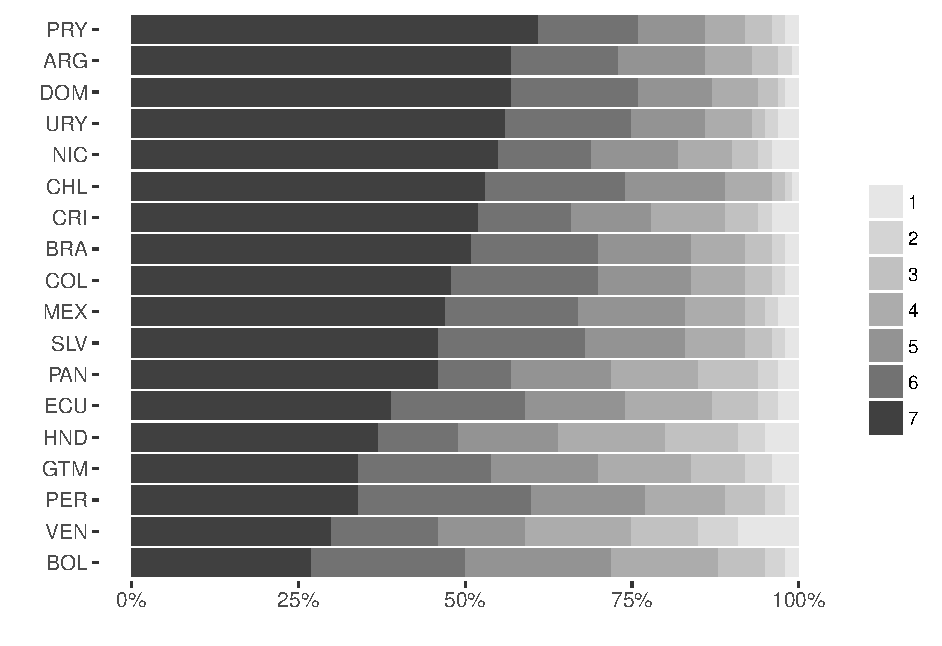
\includegraphics[width=1\textwidth]{G1.pdf}
		\caption[Acuerdo con redistribución, por países.]{Acuerdo con redistribución, por países. Porcentaje por categoría.}
		\label{fig:g1}
	\end{center}
\end{figure}

Ahora bien, ¿es el apoyo por la redistribución variable en el tiempo al interior de América Latina? ¿Qué tan estables son las preferencias en esta materia, al interior de cada país? La Figura \ref{fig:g3} responde a ello, presentando el porcentaje de personas que se identifican con los diferentes grados de acuerdo con la redistribución, por año, diferenciando según país. Como es posible observar, su comportamiento es muy diferente al interior de la región. Mientras en países como Brasil, Colombia y República Dominicana las preferencias redistributivas de las personas tienden a ser estables, casos como Bolivia, Costa Rica, Honduras y Panamá presentan notorias variaciones a lo largo del tiempo. \\

\begin{figure}[p]
	\begin{center}
		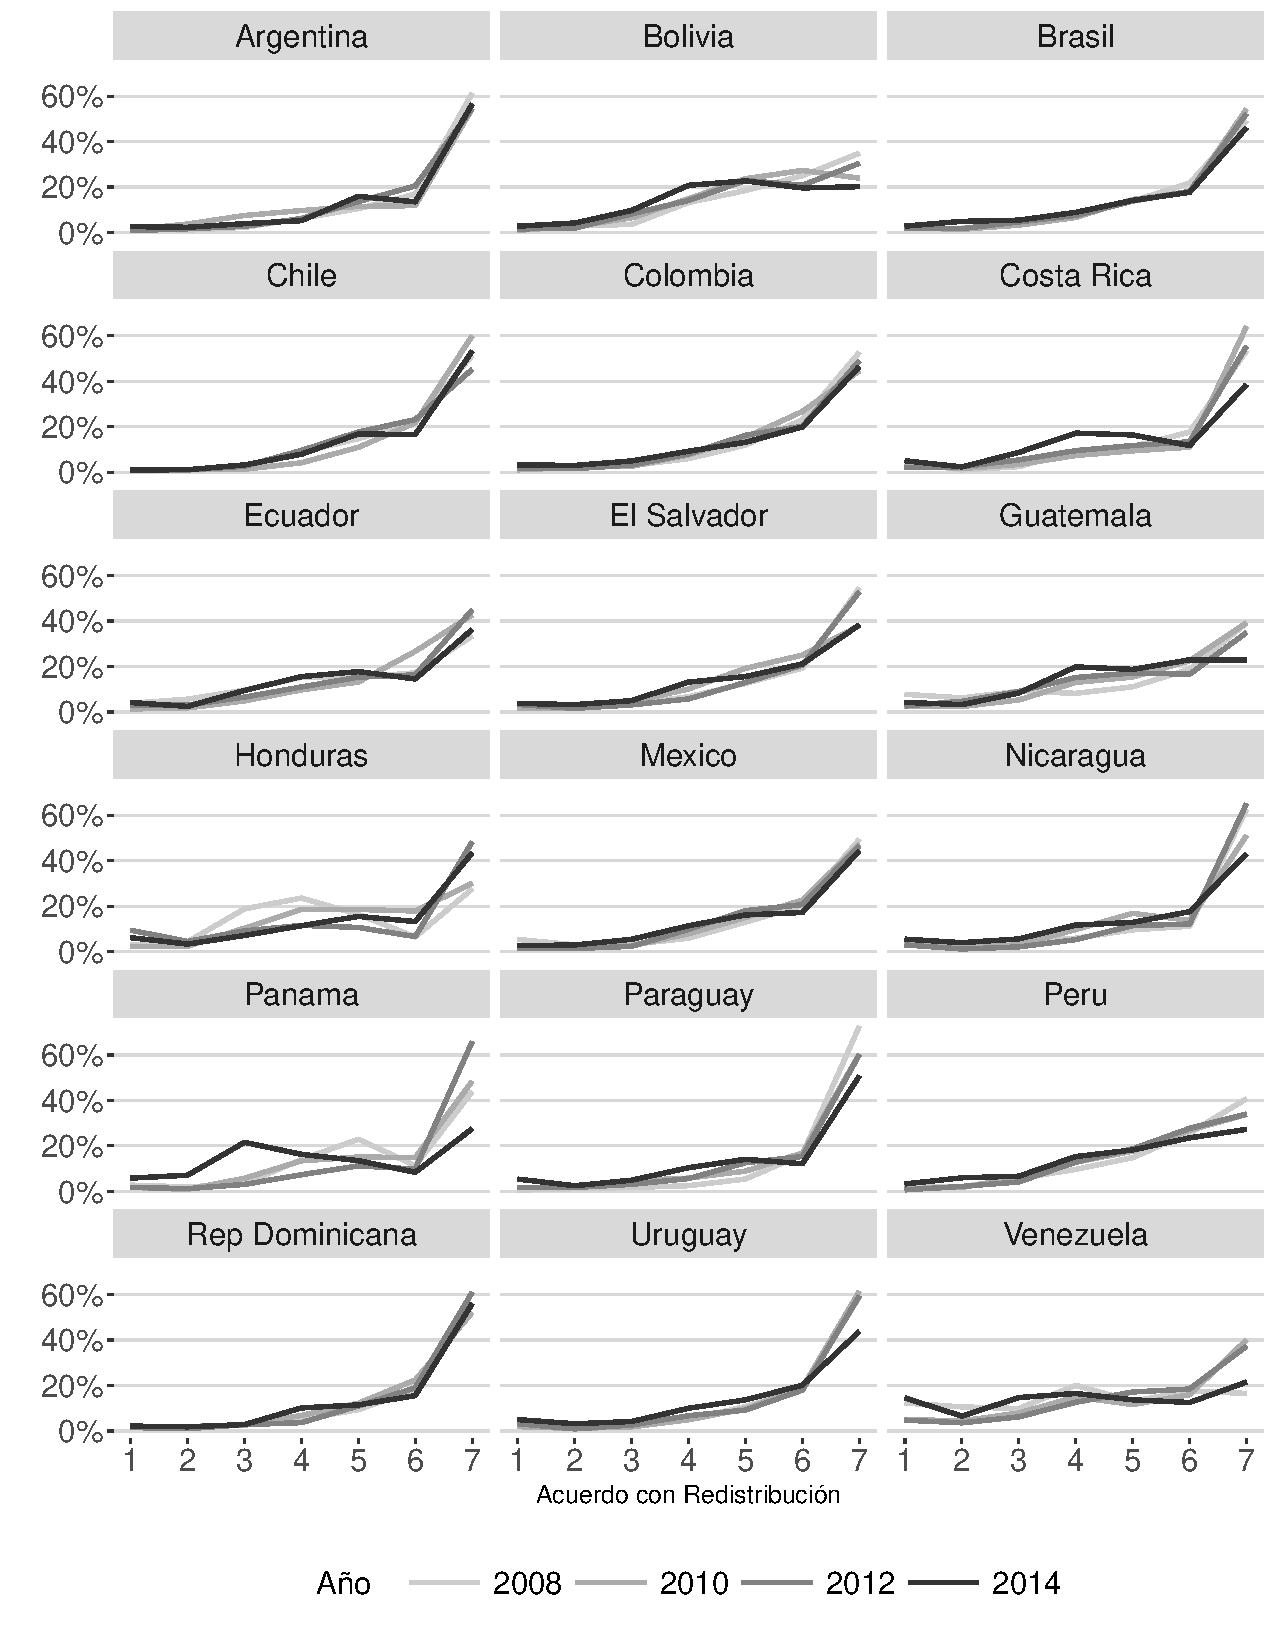
\includegraphics[width=1.05\textwidth]{G2a.pdf}
		\caption[Acuerdo con redistribución, por país y año. Porcentaje por categoría.]{Acuerdo con redistribución, por país y año. Porcentaje por categoría.}
		\label{fig:g3}
	\end{center}
\end{figure}

Otro de los aspectos centrales a evaluar es la asociación entre ingreso y preferencias redistributivas. Como se observa en la Tabla \ref{tab2}, a nivel regional, las personas de altos ingresos (quintil 5) son quienes poseen un menor apoyo por redistribución, promediando un puntaje de 5,64 en la escala de 1 a 7. Por su parte, el grupo mayormente identificado con la redistribución no es el estrato bajo (quintil 1), sino el estrato medio-bajo (quintil 2), que promedia un puntaje de 5,77. A pesar de ello, las diferencias entre quintiles tienden a ser muy reducidas.

En la mayoría de los países latinoamericanos no se cumple una relación lineal e inversa entre estrato económico y demanda por redistribución\footnote{Asimismo, esta relación presenta escasa variación a lo largo del tiempo, tomando en consideración el intervalo temporal estudiado. El detalle del grado de acuerdo con redistribución por quintil económico, según país y año se encuentra en el Anexo \ref{sec:sec66}}. A pesar de que en muchos casos el valor máximo de apoyo a la redistribución por país se presenta en un menor quintil de ingreso que para el valor mínimo, Uruguay y Venezuela son las únicas naciones donde se cumple una relación negativa lineal entre acuerdo con redistribución y quintil de ingreso. Al contrario, en la mayoría de los casos las tendencias resultan ambiguas y ambivalentes. Incluso, en países como Ecuador, El Salvador, Guatemala y República Dominicana son justamente las personas de mayores ingresos quienes expresan un mayor acuerdo con la redistribución. De esta forma, inicialmente, el análisis descriptivo rechazaría la Hipótesis H1, que establece la existencia de una relación positiva lineal entre ingreso y acuerdo con redistribución al interior de América Latina. Corresponderá testearla en adelante de forma estadística a través de los modelos híbridos de regresión.

\begin{table}[H]
	\centering
	\begin{center}
	\caption{Acuerdo con redistribución promedio según quintil de ingreso, por país}
	\label{tab2} 
    \renewcommand{\arraystretch}{0.7}
		\begin{tabular} {rrrrrrr}
			\multicolumn{ 7 }{l}{ } \cr 
			\hline
			& \textbf{Q1} & \textbf{Q2} & \textbf{Q3} & \textbf{Q4} & \textbf{Q5} & \textbf{Total} \\ 
			\hline
			Argentina & 6.05 & \textbf{6.14} & 5.96 & 5.94 & 5.93 & 6.01 \\ 
			Bolivia & 5.31 & \textbf{5.41} & 5.29 & 5.29 & 5.25 & 5.32 \\ 
			Brasil & \textbf{5.97} & 5.90 & 5.86 & 5.90 & 5.77 & 5.89 \\ 
			Chile & 6.15 & \textbf{6.24} & 5.99 & 6.08 & 5.99 & 6.10 \\ 
			Colombia & 5.89 & \textbf{5.91} & \textbf{5.91} & 5.89 & 5.90 & 5.90 \\ 
			Costa Rica & 5.73 & \textbf{5.79} & 5.71 & \textbf{5.79} & 5.70 & 5.75 \\ 
			Ecuador & 5.41 & 5.45 & \textbf{5.69} & 5.43 & 5.52 & 5.48 \\ 
			El Salvador & 5.68 & 5.85 & \textbf{5.87} & \textbf{5.87} & 5.73 & 5.80 \\ 
			Guatemala & 5.09 & 5.26 & 5.19 & 5.39 & \textbf{5.61} & 5.29 \\ 
			Honduras & \textbf{5.27} & 5.19 & 5.22 & 4.98 & 5.15 & 5.16 \\ 
			Mexico & 5.83 & 5.74 & 5.71 & \textbf{5.94} & 5.80 & 5.80 \\ 
			Nicaragua & \textbf{5.79} & 5.92 & 5.93 & 5.88 & 5.82 & 5.86 \\ 
			Panama & 5.54 & \textbf{5.63} & 5.35 & 5.52 & 5.51 & 5.53 \\ 
			Paraguay & 6.11 & 6.10 & 6.14 & \textbf{6.17} & 5.90 & 6.08 \\ 
			Peru & 5.49 & 5.61 & 5.57 & \textbf{5.62} & 5.54 & 5.56 \\ 
			Rep Dominicana & 5.99 & 6.08 & 6.09 & \textbf{6.20} & 6.13 & 6.09 \\ 
			Uruguay & \textbf{6.23} & 6.08 & 6.06 & 5.80 & 5.76 & 6.00 \\ 
			Venezuela & \textbf{5.15} & 4.91 & 4.51 & 4.77 & 4.72 & 4.87 \\ 
			\hline
			Total & 5.67 & 5.70 & 5.66 & 5.67 & 5.64 & 5.67 \\
			\hline 
			\multicolumn{7}{l}{\scriptsize{Nota: En negrita los valores máximos por país.}}
		\end{tabular}
	\end{center}
\end{table} 


\subsection{Estimación multinivel \label{sec:sec42}}

Dado el objetivo del presente estudio, corresponde analizar la distribución que posee el acuerdo con redistribución en los 18 países estudiados. La variable posee una correlación intra-clase (ICC) de 0.0368 para paises-año y de 0.0412 para países (ICC en relación a Hox, 2002, p. 32, ecuación 2.16). Esto quiere decir que de la variación en las preferencias redistributivas de las personas al interior de América Latina, un 4,12\% se debe a la pertenencia a países y un 3,68\% a países-año. Si bien parece reducida, en ningún caso inhabilita el propósito del presente estudio, dado que estos niveles de ICC son frecuentes a la hora de trabajar con países como unidades de anidación y que también se busca explicar su variación desde cuestiones a nivel individual, como el ingreso y otros.\\

La Tabla \ref{table:modelos} presenta los modelos híbridos de regresión multinivel, que estiman el acuerdo con redistribución de las personas en base a variables individuales, de países-año, países e interacciones entre niveles. El Modelo M0 es el modelo nulo, sólo anidando la varianza de la variable dependiente por país y país-año. A partir de éste, es posible estimar las ICC anteriormente señaladas. El Modelo M1 incluye al ingreso en quintiles como variable independiente; y el Modelo M2 añade, además, variables de control a nivel individual. Como se puede observar en el Modelo M1, el ingreso tendría un efecto negativo y estadísticamente significativo sobre el acuerdo por redistribución, en la misma línea de la Hipótesis H1; sin embargo, cuando se controla por otras variables influyentes sobre el acuerdo redistributivo, a través del Modelo M2, su efecto pierde toda significancia estadística. De esta forma, inicialmente, se rechazaría la Hipótesis H1, referente a una relación lineal negativa entre ingreso y acuerdo con redistribución \footnote{Tomando como evidencia el análisis descriptivo realizado en la sección anterior y las tendencias no lineales de acuerdo por redistribución a lo largo de los estratos de ingreso evidenciadas en la Tabla \ref{tab2}, se decidió estimar los Modelos M1 y M2 incluyendo el efecto cuadrático de la variable ingreso. El supuesto que estaría detrás sería que posiblemente la relación entre ingreso y acuerdo por redistribución no posea un carácter lineal, sino cuadrático, en forma de U invertida. Sin embargo, a pesar de manifestar coeficientes con significancia estadística, las magnitudes tanto de su componente lineal como cuadrático eran excesivamente reducidas, avalándose que, más allá de presentarse una verdadera relación de U invertida, con mayor acuerdo redistributivo para los estratos medios, los rangos de ingreso no presentan mayores diferencias entre sí. Para una percepción más clara del fenómeno, véase Anexo \ref{sec:sec66}.}.\\

El Modelo M3 integra todas las variables individuales incluidas en el Modelo M2 y añade además la desigualdad de los países. Esta última se encuentra descompuesta en dos dimensiones. En primer lugar, el efecto "entre" los países [BE], representado por el promedio del coeficiente Gini por país para el período estudiado (años 2008, 2010, 2012 y 2014); por esto, se constituye como una variable de nivel 3 (país). A través de ella, es posible evaluar la Hipótesis H2a, referente a la supuesta relación positiva que debiese existir entre los niveles de desigualdad y las preferencias por redistribución, entre los países. En segundo lugar, se incluye el efecto de la desigualdad "dentro de" los países [WE], relativa al cambio que presenta el coeficiente Gini de cada país-año respecto a su media país para el período estudiado. A diferencia del efecto "entre" países, esta variable varía por país-año, por lo cual es una variable a nivel 2 (país-año)\footnote{Los efectos "entre" y "dentro de" unidades tienden a abreviarse como "BE" y "WE", por su expresión en inglés "between effect" y "within effect".}.

\begin{landscape}
	
	\begin{table}
		\begin{center}
			\caption{Modelos híbridos de regresión multinivel sobre el acuerdo individual con redistribución}
			\label{table:modelos}
		    \renewcommand{\arraystretch}{0.7}
			\begin{tabular}{l D{.}{.}{5} D{.}{.}{5} D{.}{.}{5} D{.}{.}{5} D{.}{.}{5} D{.}{.}{5} D{.}{.}{5} D{.}{.}{5} D{.}{.}{5} }
				\hline
				& \multicolumn{1}{c}{\textbf{M0}} & \multicolumn{1}{c}{\textbf{M1}} & \multicolumn{1}{c}{\textbf{M2}} & \multicolumn{1}{c}{\textbf{M3}} & \multicolumn{1}{c}{\textbf{M4}} & \multicolumn{1}{c}{\textbf{M5}} & \multicolumn{1}{c}{\textbf{M6}} & \multicolumn{1}{c}{\textbf{M7}} & \multicolumn{1}{c}{\textbf{M8}} \\ \hline
				\textit{Var. individuales} &                        &                        &                        &                        &                        &                        &                        &                        &                        \\
				Ingreso                    &                        & -0.01^{**}             & -0.01                  & -0.01                  & -0.01                  & -0.01                  & -0.01                  & -0.22                  & 0.05^{*}               \\
				&                        & (0.00)                 & (0.00)                 & (0.00)                 & (0.00)                 & (0.00)                 & (0.01)                 & (0.14)                 & (0.03)                 \\
				Hombre                     &                        &                        & 0.05^{***}             & 0.05^{***}             & 0.05^{***}             & 0.05^{***}             & 0.05^{***}             & 0.05^{***}             & 0.05^{***}             \\
				&                        &                        & (0.01)                 & (0.01)                 & (0.01)                 & (0.01)                 & (0.01)                 & (0.01)                 & (0.01)                 \\
				Edad                       &                        &                        & 0.00                   & 0.00                   & 0.00                   & 0.00                   & 0.00                   & 0.00                   & 0.00                   \\
				&                        &                        & (0.00)                 & (0.00)                 & (0.00)                 & (0.00)                 & (0.00)                 & (0.00)                 & (0.00)                 \\
				Casado                     &                        &                        & 0.04^{***}             & 0.04^{***}             & 0.04^{***}             & 0.04^{***}             & 0.04^{***}             & 0.04^{***}             & 0.04^{***}             \\
				&                        &                        & (0.01)                 & (0.01)                 & (0.01)                 & (0.01)                 & (0.01)                 & (0.01)                 & (0.01)                 \\
				Izquierda                  &                        &                        & 0.01^{***}             & 0.01^{***}             & 0.01^{***}             & 0.01^{***}             & 0.01^{***}             & 0.01^{***}             & 0.01^{***}             \\
				&                        &                        & (0.00)                 & (0.00)                 & (0.00)                 & (0.00)                 & (0.00)                 & (0.00)                 & (0.00)                 \\
				Confianza                  &                        &                        & 0.08^{***}             & 0.08^{***}             & 0.08^{***}             & 0.08^{***}             & 0.08^{***}             & 0.08^{***}             & 0.08^{***}             \\
				&                        &                        & (0.00)                 & (0.00)                 & (0.00)                 & (0.00)                 & (0.00)                 & (0.00)                 & (0.00)                 \\
				S.L. Desempleado           &                        &                        & 0.04^{**}              & 0.04^{**}              & 0.04^{**}              & 0.04^{**}              & 0.04^{**}              & 0.04^{**}              & 0.04^{**}              \\
				&                        &                        & (0.02)                 & (0.02)                 & (0.02)                 & (0.02)                 & (0.02)                 & (0.02)                 & (0.02)                 \\
				S.L. Empleado              &                        &                        & 0.02                   & 0.02                   & 0.02                   & 0.02                   & 0.02                   & 0.02                   & 0.02                   \\
				&                        &                        & (0.02)                 & (0.02)                 & (0.02)                 & (0.02)                 & (0.02)                 & (0.02)                 & (0.02)                 \\
				Ed. Secundaria             &                        &                        & 0.04^{**}              & 0.04^{**}              & 0.04^{**}              & 0.04^{**}              & 0.03^{**}              & 0.03^{**}              & 0.03^{**}              \\
				&                        &                        & (0.01)                 & (0.01)                 & (0.01)                 & (0.01)                 & (0.01)                 & (0.01)                 & (0.01)                 \\
				Ed. Terciaria              &                        &                        & 0.02                   & 0.02                   & 0.02                   & 0.02                   & 0.03                   & 0.03                   & 0.03                   \\
				&                        &                        & (0.02)                 & (0.02)                 & (0.02)                 & (0.02)                 & (0.02)                 & (0.02)                 & (0.02)                 \\
				Urbano                     &                        &                        & -0.03^{**}             & -0.03^{**}             & -0.03^{**}             & -0.03^{**}             & -0.04^{***}            & -0.04^{***}            & -0.04^{***}            \\
				&                        &                        & (0.01)                 & (0.01)                 & (0.01)                 & (0.01)                 & (0.01)                 & (0.01)                 & (0.01)                 \\ \hline
				\multicolumn{10}{l}{\scriptsize{$^{***}p<0.01$, $^{**}p<0.05$, $^*p<0.1$}}
			\end{tabular}
		\end{center}
	\end{table}
	
	\newpage
	
	\begin{table}
		\begin{center}
	    \renewcommand{\arraystretch}{0.7}
			\begin{tabular}{l D{.}{.}{5} D{.}{.}{5} D{.}{.}{5} D{.}{.}{5} D{.}{.}{5} D{.}{.}{5} D{.}{.}{5} D{.}{.}{5} D{.}{.}{5} }
				\hline
				& \multicolumn{1}{c}{\textbf{M0}} & \multicolumn{1}{c}{\textbf{M1}} & \multicolumn{1}{c}{\textbf{M2}} & \multicolumn{1}{c}{\textbf{M3}} & \multicolumn{1}{c}{\textbf{M4}} & \multicolumn{1}{c}{\textbf{M5}} & \multicolumn{1}{c}{\textbf{M6}} & \multicolumn{1}{c}{\textbf{M7}} & \multicolumn{1}{c}{\textbf{M8}} \\ \hline
				\textit{Var. país}            &                        &                        &                        &                        &                        &                        &                        &                        &                        \\
				Gini [BE]                     &                        &                        &                        & 0.01                   & 0.02                   & 0.01                   & 0.01                   & 0.01                   & 0.01                   \\
				&                        &                        &                        & (0.02)                 & (0.02)                 & (0.02)                 & (0.02)                 & (0.02)                 & (0.02)                 \\
				Gini [WE]                     &                        &                        &                        & -0.00                  & -0.00                  & -0.00                  & -0.01                  & -0.01                  & -0.01                  \\
				&                        &                        &                        & (0.02)                 & (0.02)                 & (0.02)                 & (0.02)                 & (0.02)                 & (0.02)                 \\
				PIB [BE]                      &                        &                        &                        &                        & 0.03                   & 0.00                  & 0.04^{*}               & 0.04^{*}               & 0.06^{**}              \\
				&                        &                        &                        &                        & (0.02)                 & (0.05)                 & (0.02)                 & (0.02)                 & (0.02)                 \\
				PIB [WE]                      &                        &                        &                        &                        & -0.16^{**}             & -0.16^{**}             & -0.13^{*}              & -0.13^{*}              & -0.14^{*}                  \\
				&                        &                        &                        &                        & (0.08)                 & (0.08)                 & (0.08)                 & (0.08)                 & (0.08)                 \\
				E. Productivista              &                        &                        &                        &                        &                        & 0.45                   &                        &                        &                        \\
				&                        &                        &                        &                        &                        & (0.46)                 &                        &                        &                        \\
				E. Proteccionista             &                        &                        &                        &                        &                        & 0.20                   &                        &                        &                        \\
				&                        &                        &                        &                        &                        & (0.34)                 &                        &                        &                        \\
				\textit{Interac. inter-nivel} &                        &                        &                        &                        &                        &                        &                        &                        &                        \\
				Ingreso * Gini[BE]            &                        &                        &                        &                        &                        &                        &                        & 0.00                   &                        \\
				&                        &                        &                        &                        &                        &                        &                        & (0.00)                 &                        \\
				Ingreso * Gini[WE]            &                        &                        &                        &                        &                        &                        &                        & -0.00                   &                        \\
				&                        &                        &                        &                        &                        &                        &                        & (0.00)                 &                        \\
				Ingreso * PIB[BE]             &                        &                        &                        &                        &                        &                        &                        &                        & -0.01^{**}             \\
				&                        &                        &                        &                        &                        &                        &                        &                        & (0.00)                 \\
				Ingreso * PIB[WE]             &                        &                        &                        &                        &                        &                        &                        &                        & 0.00                   \\
				&                        &                        &                        &                        &                        &                        &                        &                        & (0.02)                 \\
				\textit{Tend. temporales}    &                        &                        &                        &                        &                        &                        &                        &                        &                        \\
				2010                          &                        & 0.08                   & 0.06                   & 0.06                   & 0.08                   & 0.08                   & 0.07                   & 0.07                   & 0.07                   \\
				&                        & (0.08)                 & (0.08)                 & (0.09)                 & (0.08)                 & (0.08)                 & (0.08)                 & (0.08)                 & (0.08)                 \\
				2012                          &                        & 0.11                   & 0.09                   & 0.09                   & 0.18^{*}               & 0.18^{*}               & 0.14                   & 0.14                   & 0.14                   \\
				&                        & (0.08)                 & (0.08)                 & (0.10)                 & (0.11)                 & (0.11)                 & (0.10)                 & (0.10)                 & (0.10)                 \\
				2014                          &                        & -0.32^{***}            & -0.33^{***}            & -0.33^{***}            & -0.19                  & -0.19                  & -0.27^{**}             & -0.27^{**}             & -0.27^{**}             \\
				&                        & (0.08)                 & (0.08)                 & (0.10)                 & (0.12)                 & (0.12)                 & (0.11)                 & (0.11)                 & (0.11)                 \\
				(Intercepto)                  & 5.69^{***}             & 5.75^{***}             & 5.26^{***}             & 4.57^{***}             & 4.12^{***}             & 4.49^{***}             & 4.26^{***}             & 4.64^{***}             & 4.17^{***}             \\
				& (0.09)                 & (0.10)                 & (0.10)                 & (0.91)                 & (0.91)                 & (1.04)                 & (0.90)                 & (0.93)                 & (0.90)                 \\ \hline
				\multicolumn{10}{l}{\scriptsize{$^{***}p<0.01$, $^{**}p<0.05$, $^*p<0.1$}}
			\end{tabular}
		\end{center}
	\end{table}
	
	\newpage
	
	\begin{table}
		\begin{center}
	    \renewcommand{\arraystretch}{0.7}
			\begin{tabular}{l c{5} c{5} c{5} c{5} c{5} c{5} c{5} c{5} c{5}}
				\hline
				& \multicolumn{1}{c}{\textbf{M0}} & \multicolumn{1}{c}{\textbf{M1}} & \multicolumn{1}{c}{\textbf{M2}} & \multicolumn{1}{c}{\textbf{M3}} & \multicolumn{1}{c}{\textbf{M4}} & \multicolumn{1}{c}{\textbf{M5}} & \multicolumn{1}{c}{\textbf{M6}} & \multicolumn{1}{c}{\textbf{M7}} & \multicolumn{1}{c}{\textbf{M8}} \\ \hline
				\textit{Ajuste y varianza} &             &             &             &             &             &             &             &             &             \\
				AIC                                   & 307541  & 307535   & 307170   & 307185   & 307192  & 307196  & 306933   & 306954   & 306948   \\
				BIC                                   & 307578  & 307610   & 307337   & 307371   & 307397  & 307419  & 307176   & 307215   & 307209   \\
				Log Likelihood                       & -153766 & -153760  & -153567  & -153572  & -153574 & -153574 & -153440  & -153449  & -153446  \\
				N Nivel 1                            & 82866      & 82866       & 82866       & 82866       & 82866      & 82866      & 82866       & 82866       & 82866       \\
				N Nivel 2                & 72         & 72          & 72          & 72          & 72         & 72         & 72          & 72          & 72          \\
				N Nivel 3                    & 18         & 18          & 18          & 18          & 18         & 18         & 18          & 18          & 18          \\
				Var: N2 (Int)            & 0.10       & 0.06        & 0.06        & 0.06        & 0.06       & 0.06       & 0.06        & 0.06        & 0.06        \\
				Var: N3 (Int)                & 0.11       & 0.12        & 0.11        & 0.12        & 0.11       & 0.12       & 0.11        & 0.11        & 0.11        \\
				Var: Residual                        & 2.39       & 2.39        & 2.37        & 2.37        & 2.37       & 2.37       & 2.36        & 2.36        & 2.36        \\
				Var: N2 Ingreso             &            &             &             &             &            &            & 0.00        & 0.00        & 0.00        \\
				Cov: N2 (Int) Ingreso &            &             &             &             &            &            & -0.01       & -0.01       & -0.01       \\
				Var: N3 Ingreso                 &            &             &             &             &            &            & 0.00        & 0.00        & 0.00        \\
				Cov: N3 (Int) Ingreso     &            &             &             &             &            &            & -0.00       & -0.00       & -0.00       \\
				\hline
				\multicolumn{10}{l}{\scriptsize{$^{***}p<0.01$, $^{**}p<0.05$, $^*p<0.1$}}
			\end{tabular}
		\end{center}
	\end{table}
	
\end{landscape}


Como se observa en la Tabla \ref{table:modelos}, tanto el Gini [BE] como el Gini [WE] presentan efectos con magnitudes casi inexistentes y no logran configurarse como estadísticamente significativos; fenómeno que se evidencia en los Modelos M3 y M4. De esta forma, se corrobora la ausencia de patrones estables entre desigualdad y acuerdo por redistribución\footnote{Para una representación gráfica de ello, ver Anexos \ref{sec:sec62} y \ref{sec:sec63}}. En otras palabras, se confirma que al interior de América Latina, los niveles y los cambios en la desigualdad de los países no generan consecuencias sobre el apoyo de las personas hacia la redistribución, rechazándose así las Hipótesis H2a y H2b, respectivamente.\\

El Modelo M4, por su parte, incluye el efecto del desarrollo económico sobre el acuerdo individual con la redistribución, tanto "entre" como "dentro de" los países. En éste, es posible observar que los niveles de desarrollo de los países no manifestarían mayor injerencia sobre la variable dependiente, mostrándose su coeficiente como no significativo. Sin embargo, su cambio en el tiempo sí lo haría: el aumento en mil dólares del PIB per cápita en el tiempo se asocia a una disminución  de 0.16 puntos en el acuerdo individual por redistribución, significativo a un 90\% de confianza.\\

El Modelo M5 se estima con el objetivo de evaluar el efecto de la desigualdad y el desarrollo, controlando por la "heterogeneidad no observada" que afectaría sobre las preferencias por redistribución de forma diferenciada entre los países, según el tipo de régimen de bienestar (Schmidt-Catran, 2016). Recordemos que esta clasificación contempla 3 categorías\footnote{Productivistas, proteccionistas e informales familiares} y, en este caso, la categoría de referencia son los regímenes "informales familiares", escasamente desarrollados en materia de bienestar y protección social al interior de América Latina (Martínez Franzoni, 2008). Como se puede apreciar en la Tabla \ref{table:modelos}, la inclusión de la tipología de regímenes no genera modificaciones estadísticas en los efectos de la desigualdad y el desarrollo, continuando no significativos y bajos en términos de magnitud. Por ello y apelando a una mayor parsimonia, en adelante se estiman los modelos sin su presencia.\\

El Modelo M6 trabaja con el ingreso, las variables individuales de control, la desigualdad y la riqueza de los países; estas últimas en sus versiones "entre" y "dentro de" países. La diferencia con respecto al Modelo M4 es que incorpora pendientes aleatorias por país-año y país para el efecto del ingreso. En concreto, el Modelo M6 permite que la relación entre los quintiles de ingreso y el apoyo hacia la redistribución varíe por país-año (nivel 2) y país (nivel 3). Como es posible observar, aún controlándose por el coeficiente Gini y el PIB per cápita de los países, el efecto del ingreso se mantiene no significativo. Así, se reafirma el rechazo de la Hipótesis H1, que avalaba una relación negativa entre el estrato de ingreso del individuo y su apoyo a la reducción de brechas económicas por parte del Estado. Al interior de América Latina, el ingreso de las personas, por sí sólo, no se constituye como un determinante influyente sobre el acuerdo con la redistribución.\\

A pesar de ello, importante es ahondar en las diferencias que podrían existir a lo largo de los países de la región, respecto a la relación existente entre la posición socioeconómica objetiva de las personas y sus preferencias en materia redistributiva. Por ello, la Figura \ref{fig:ingaleatorio} da cuenta del efecto aleatorio de la variable ingreso sobre el acuerdo redistributivo por país, en términos de su intercepto (quintil 1), como de su pendiente (cambio por el aumento en un quintil de ingreso); todo esto calculado en base al Modelo M6. Como se mencionó anteriormente, en la región el ingreso no expresa diferencias significativas sobre el apoyo por redistribución; sin embargo, cada país se comporta de forma diferente en este ámbito. \\

\begin{figure}
	\centering
	\begin{tabular}{cc}
		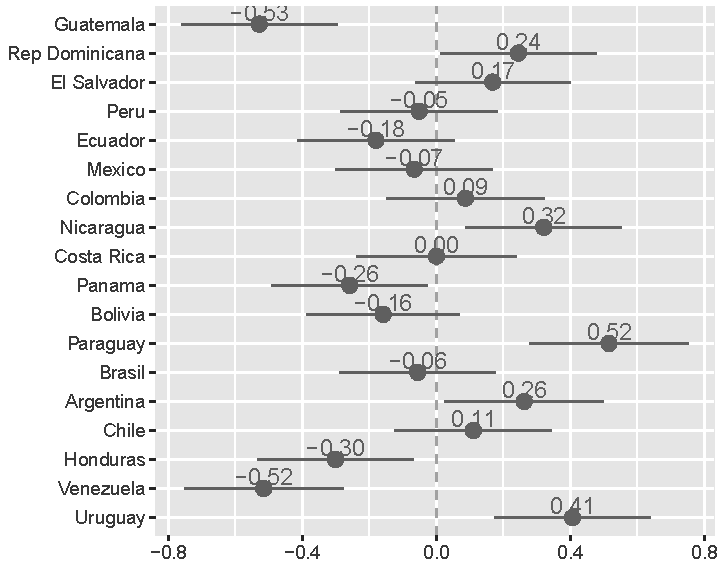
\includegraphics[width=0.54\textwidth]{Pend_Int02.pdf} & 
		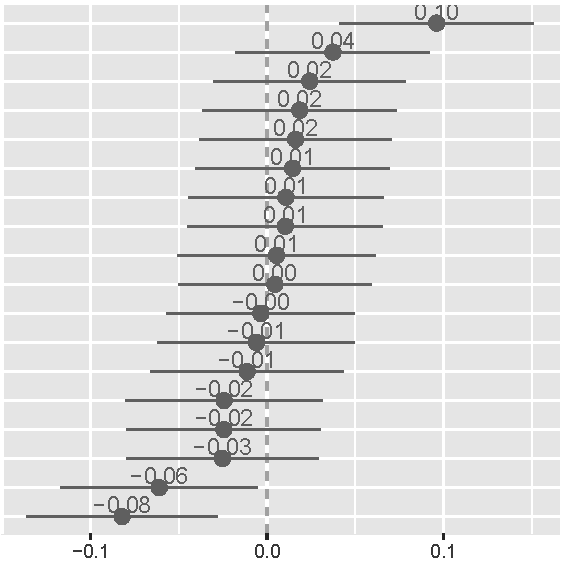
\includegraphics[width=0.422\textwidth]{Pend_Ing02.pdf}
	\end{tabular}
	\caption{Efecto aleatorio de Ingreso sobre Acuerdo con Redistribución por país: intercepto y pendiente}
	\label{fig:ingaleatorio}
\end{figure}

La Figura \ref{fig:ingaleatorio} evidencia que ocho países presentan una relación negativa entre quintil de ingreso y demanda por redistribución y diez una de carácter positiva; sin embargo, en sólo tres de los 18 países el ingreso posee un efecto estadísticamente significativo a un 95\% de confianza (ver pendientes en Figura \ref{fig:ingaleatorio}). Así, es posible afirmar que Venezuela y Uruguay son los únicos dos países en donde se evidencia la Hipótesis H1 y la influencia del autointerés: en dichas naciones, a medida que las personas son más ricas, prefieren una menor redistribución de recursos; sin embargo, ambos con interceptos o "puntos de partida" radicalmente diferentes. Mientras en Uruguay el quintil más pobre se asocia a un incremento en el acuerdo redistributivo, en Venezuela éste tiene un efecto negativo, evidenciando que en dicha nación, independiente del estrato económico, las personas siempre tenderán a manifestar un menor acuerdo redistributivo que sus pares regionales. Caso contrario ocurre en Guatemala, donde se expresa una relación positiva: a medida que las personas son más ricas, mayor es su acuerdo con la disminución de brechas socioeconómicas vía la acción del Estado. En el resto de los países no es posible establecer conclusiones significativas.\\

Asimismo, el Modelo M6 avala con un 90\% de confianza que el mero hecho de pertenecer a un país más rico en mil dólares per cápita, se asocia a un incremento de 0.04 puntos de acuerdo con la redistribución. Podría parecer ínfima la cifra, pero no deja de ser importante tomando en consideración la diversidad que presenta la región en materia de riquezas económicas nacionales: considerando los cuatro años estudiados, Nicaragua -el más pobre- presenta un PIB promedio de 1.632 dólares, mientras que Chile -el más rico- uno de 13.395 dólares. Lo que manifiesta este coeficiente, es que sólo por el efecto del nivel de desarrollo económico de los países, los chilenos poseerán un apoyo 0.47 puntos mayor que los nicaragüenses, en la escala de acuerdo redistributivo que oscila de 1 a 7. \\

Sin embargo, este efecto se contrapone con el que expresa el cambio en el PIB dentro de cada país en el tiempo (PIB [WE]). Éste establece que a medida que los países manifiestan un aumento de su riqueza en mil dólares per cápita, las personas tenderán a expresar una baja de 0.13 puntos en su grado de acuerdo con la disminución de desigualdades. Por ello, los habitantes de países más ricos tenderán a ser más redistributivos pero, paradójicamente, el incremento del PIB per cápita en el tiempo los hará menos favorables a la redistribución. Así, el desarrollo económico expresa un efecto contracíclico, que comprueba la Hipótesis H4a, pero rechaza la Hipótesis H4b, existiendo una discrepancia entre los efectos asociados al nivel y al cambio en el desarrollo de las naciones.\\

Los Modelos M7 y M8, presentes en la Tabla \ref{table:modelos}, añaden interacciones entre niveles: el primero, establece una interacción entre el ingreso y la desigualdad de los países, tanto respecto al nivel como al cambio en el tiempo; y el segundo, realiza lo mismo, sólo que con relación al desarrollo económico de las naciones. Como se evidencia en el Modelo M7 tanto el nivel como el cambio de la desigualdad no generan modificaciones en la relación que manifiesta el quintil de ingreso de las personas y su apoyo hacia la acción redistributiva del Estado. Ambos coeficientes, Gini [BE] y Gini [WE], son nulos tanto en magnitud como en significancia estadística. En caso que la Hipótesis H3 hubiese sido cierta, dichos coeficientes serían negativos, por tanto es posible rechazarla: la desigualdad no genera cambios en la relación del ingreso de las personas y su acuerdo con la redistribución.\\

Con respecto al desarrollo sí se evidencian hallazgos relevantes. En el Modelo M8, la interacción entre desarrollo económico e ingreso alberga poder explicativo, en tanto los cinco coeficientes involucrados (Ingreso, PIB [BE], PIB [WE], Ingreso * PIB [BE] e Ingreso * PIB [WE]) tienden a alcanzar significancia estadística. La interpretación que se desprende de aquellos es la siguiente. En primer lugar, se afirma que para los países pobres, con un PIB hipotéticamente nulo, el incremento en un estrato de ingreso se asocia a un alza en el acuerdo con redistribución de 0.05 puntos a un 90\% de confianza. Sin embargo, dicho efecto del ingreso comienza a disminuir para los países más ricos, en una razón de 0.01 puntos menos de acuerdo redistributivo por el aumento en mil dólares del PIB per cápita nacional. Y dado que el PIB promedio en el período oscila entre 1,6 (Nicaragua) y 13,4 (Chile), pasado un nivel de desarrollo, el efecto del ingreso comienza a ser negativo, evidenciándose mayores diferencias entre los estratos económicos, siendo los quintiles más ricos significativamente más adversos a la redistribución en países ricos. Así, en sociedades económicamente más desarrolladas, el ingreso manifiesta una relación negativa cada vez más fuerte con las preferencias por redistribución. El cambio de la riqueza "dentro de" los países, asimismo, no expresa efectos significativos sobre la relación del ingreso con las preferencias redistributivas.\\

Los hechos recién descritos se manifiestan con mayor claridad por medio de la Figura \ref{fig:interac}. En ella se presentan los efectos condicionales del ingreso sobre el acuerdo redistributivo, según los niveles y cambios, tanto de la desigualdad como la riqueza de los países\footnote{Intervalos a un nivel de confianza del 90\%.} (Modelos M7 y M8, respectivamente). Con respecto a la desigualdad, se confirma la ausencia de pendiente negativa, como la Hipótesis H3 intentaba sugerir. Para el rol "entre" países, vinculado a los promedios del coeficiente Gini, se observa una pendiente positiva pero nunca significativa, por lo cual no es posible avalar un efecto de la desigualdad en la relación entre ingreso y acuerdo con redistribución. Respecto al cambio en desigualdad de los países, la pendiente es nula y nunca alcanza valores significativos, por lo cual su efecto es inexistente. Se refuta, así, la Hipótesis H3, referente al rol atenuante que pudiese tener el incremento de la desigualdad de los países sobre las diferencias entre estratos económicos en materia redistributiva al interior de América Latina.\\

Sin embargo, lo que sí es trascendental, es la evidencia que la Figura \ref{fig:interac} hace respecto al rol moderador del desarrollo económico sobre la relación entre ingreso y acuerdo con la redistribución, manifiesto a través del Modelo M8. Como se mencionó previamente, un mayor desarrollo económico se asocia a un efecto cada vez más negativo entre el ingreso de las personas y su apoyo hacia la reducción de desigualdades vía la acción estatal, el cual alcanza significancia estadística sobre los 10 mil dólares anuales de PIB per cápita. Si bien el efecto del cambio en el tiempo de la riqueza nacional no expresa modificaciones en la relación analizada, es posible avalar la Hipótesis H5: en los países con mayor desarrollo económico, la relación entre el ingreso y el acuerdo individual con la redistribución es más fuerte que en países menos desarrollados, siendo los estratos ricos más adversos hacia la disminución de desigualdades que los estratos pobres.

\begin{figure}[H]
	\centering
	\begin{tabular}{cc}
		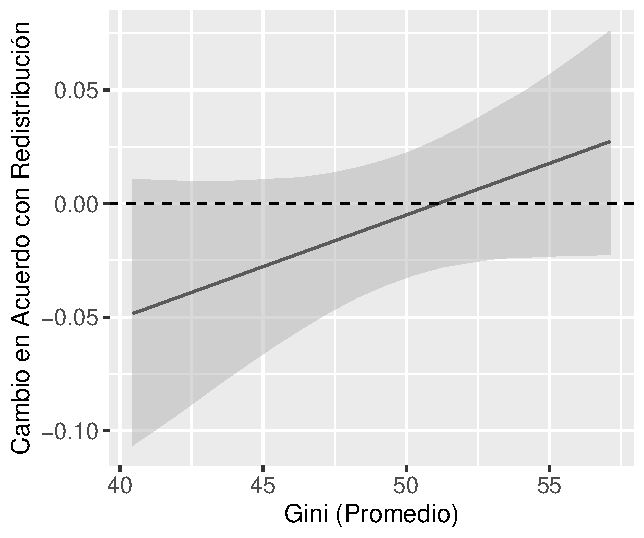
\includegraphics[width=0.49\textwidth]{MarGINI1.pdf} & 
		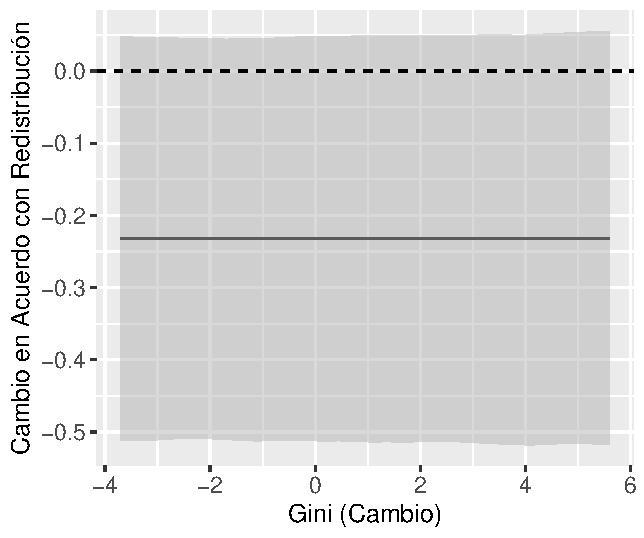
\includegraphics[width=0.49\textwidth]{MarGINI2.pdf} \\
		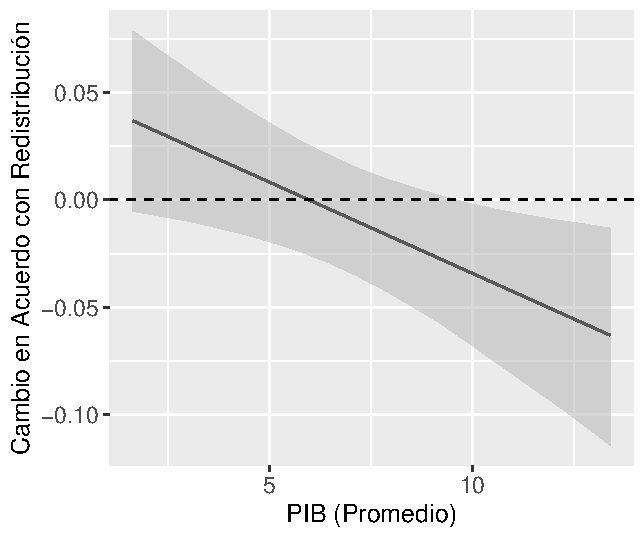
\includegraphics[width=0.49\textwidth]{MarPIB1.pdf} & 
		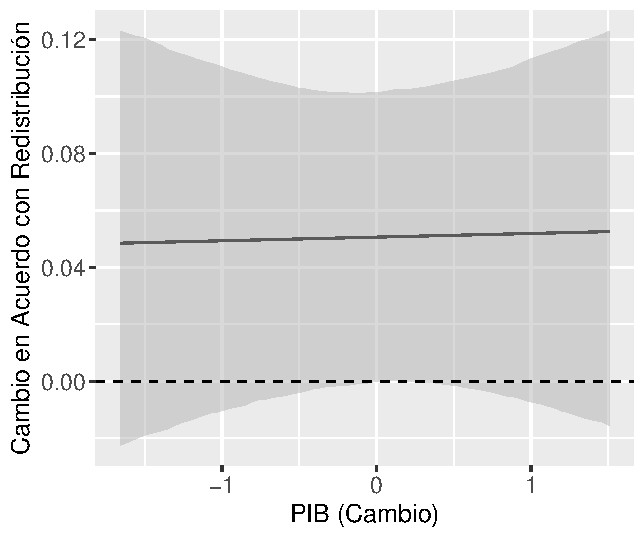
\includegraphics[width=0.49\textwidth]{MarPIB2.pdf} 
	\end{tabular}
	\caption{Efecto condicional de Ingreso sobre Acuerdo con Redistribución. Interacciones inter-nivel.}
	\label{fig:interac}
\end{figure}

Respecto al resto de variables individuales, incluidas para controlar el testeo de las hipótesis establecidas, es posible resaltar hallazgos no menores. En primer lugar, como se observa a lo largo de la Tabla \ref{table:modelos}, la totalidad de las variables individuales se comporta de forma constante a lo largo de los modelos estimados, tanto en términos de magnitud como significancia. Por lo mismo, es posible establecer con seguridad que, al interior de América Latina, los hombres, las personas casadas, desempleadas y con educación secundaria (respeto a quienes poseen al menos enseñanza básica completa), además de los residentes en zonas rurales, poseen un mayor acuerdo con la redistribución.\\

A pesar de esto, existe un determinante en particular que requiere ser resaltado con principal detención, por constituirse como el más influyente de la totalidad de características a nivel individual evaluadas: la confianza en el sistema político. Significativa a un 99\% de confiabilidad, el incremento en un punto de confianza en el sistema por parte de las personas se asocia a un aumento en 0.08 puntos en su acuerdo con la redistribución. Al oscilar esta variable entre los 1 y 7 puntos, la diferencia entre una persona totalmente desconfiada del sistema y otra completamente confiada, asciende a cerca de 0.5 puntos en el acuerdo por redistribución; un efecto tremendamente relevante, que resalta el poder que tiene la confianza en el Estado sobre las preferencias redistributivas de la población latinoamericana.\\

Finalmente, tomando en consideración la naturaleza longitudinal del presente estudio, se evidencia un fenómeno que no deja de ser importante y que requiere ser abordado. Como bien expresa la Tabla \ref{table:modelos}, se tiende a no evidenciar variaciones temporales, con la principal excepción del año 2014, altamente negativo y significativo a un 99\% de confianza en la mayoría de los modelos estimados. Así, si se toma como referencia el Modelo M6, en 2014 la población latinoamericana tendió a manifestar una baja significativa de 0.27 puntos respecto a 2008 en su acuerdo por redistribución, controlando por la totalidad de factores a nivel individual, así como los niveles y cambios de la desigualdad y riqueza de las naciones.

\newpage

\section{CONCLUSIONES}

Los resultados del presente estudio ponen en entredicho a las aproximaciones hegemónicas en preferencias redistributivas, basadas en el autointerés, así como sus pretensiones universalistas. A diferencia de lo que se ha tendido a plantear en otros contextos, los resultados afirman la inexistencia de una relación entre el ingreso de las personas y su acuerdo con la redistribución de recursos. En otras palabras, en regiones desiguales y en vías de desarrollo, como América Latina, el estrato económico al que pertenecen los individuos no se configura como un determinante influyente sobre su demanda por la reducción de desigualdades. En línea con lo planteado por Dion \& Birchfield (2010), las particularidades de la región refutan el hecho que las personas elaboren sus preferencias redistributivas en torno a la maximización de utilidades asociadas y la relación entre costos y beneficios.\\

Sin embargo, por sobre negar de raíz dichas formulaciones racionalistas, el presente estudio especifica su campo de acción, resaltando la importancia que poseen las particularidades del contexto en el cual se sitúan las personas. Y es que si bien se ha dicho que en nuestra región el ingreso no se constituye como un determinante transversal, sí posee espacios en su interior donde éste emerge como un factor explicativo. Como se avala a través de los modelos de regresión estimados, el principal gatillante de su influencia en América Latina sería el desarrollo económico de los países. Si bien al interior de naciones mayormente empobrecidas, las personas no diferencian sus preferencias según el estrato económico al que pertenecen, en países ricos sí es posible visualizar dicha relación negativa entre ingreso y acuerdo con la redistribución. De ahí se explica la evidencia contrapuesta que poseen los hallazgos del presente estudio con los reportados por Schmidt-Catran (2016) en contexto europeo.\\

Los hallazgos, en la misma línea de Bowles \& Gintis (2000), avalan la participación que ejercen ciertas consideraciones morales sobre el prójimo y la importancia que alberga el asegurar la provisión de estándares mínimos de existencia para los demás, en la definición de actitudes hacia la redistribución. En contextos nacionales más empobrecidos, donde la satisfacción de necesidades básicas no se encuentra del todo cubierta, este tipo de evaluaciones dejaría en un segundo plano al autointerés propio de la condición estructural de las personas. Así, la diversidad de niveles de desarrollo económico existente a lo largo de los países que conforman la región, generaría diferencias en las formas en que el ingreso expresa efectos sobre las preferencias redistributivas, emergiendo en contextos más ricos y ocultándose entre naciones menos desarrolladas. \\

La ausencia del autointerés en sociedades económicamente sub-desarrolladas al interior de América Latina daría cuenta de la presencia de una solidaridad social cargada moralmente por una preocupación hacia el otro, en línea de lo que la literatura ha entendido como "Homo reciprocans". Según Bowles \& Gintis (2000), este tipo ideal "se preocupa por el bienestar de los demás y por el proceso de determinación de los resultados; difiere en esto del Homo economicus preocupado de sí mismo y orientado a resultados" (p. 37). Así, el desarrollo económico dentro de la región sería clave a la hora de articular diferentes tipos de solidaridad social al interior de las sociedades, materializada en última instancia sobre el acuerdo que las personas expresan hacia la redistribución de recursos y el grado en que éste último se ve determinado por la posición objetiva en la estructura social, junto a la consiguiente evaluación racional de costos y beneficios individuales producidos por la redistribución.\\

También respecto al accionar de la riqueza de los países, particular resulta lo que se denominó anteriormente como el "efecto contracíclico del desarrollo", referente a las influencias contrapuestas que genera la diferencia del PIB per cápita "entre" y "dentro de" los países. Como mostraron los modelos híbridos de regresión, las naciones más desarrolladas al interior de la región se encuentran asociadas a mayores niveles de demanda por redistribución; sin embargo, el enriquecimiento de las naciones a lo largo del tiempo conlleva, asimismo, una contracción de dicha demanda. La emergencia de efectos en dirección contraria por parte del desarrollo podría estar avalando un efecto de "path-dependence" donde, a pesar de que el crecimiento económico se asocie a menores probabilidades de acuerdo con la redistribución, los ciudadanos de naciones más ricas se mantendrán más propensos a la redistribución por la experiencia de un contexto de necesidades existenciales mayormente cubiertas, terreno fértil para la emergencia de valores postmaterialistas (Inglehart, 2008), antagónicos al cálculo egoísta (Gelissen, 2000). Aun así, este fenómeno requiere ser estudiado con mayor detención para comprender realmente aquello que quiere expresar para nuestra región.\\

Asimismo, la ausencia de efecto por parte de la desigualdad podría explicarse por la divergencia, empíricamente comprobada en muchos contextos, entre desigualdad objetiva y subjetiva (J. C. Castillo, 2010; Sachweh \& Olafsdottir, 2012). Más que los cambios en los niveles reales de desigualdad, lo que realmente podría generar modificaciones en el acuerdo con la redistribución serían las percepciones, creencias y juicios hacia la desigualdad (Janmaat, 2013), preponderantes en cada uno de los países. Según Cramer \& Kaufman (2011) las diferencias entre estratos de ingreso respecto a la insatisfacción con la desigualdad existente, en América Latina, tampoco se ven potenciadas cuando los niveles de desigualdad objetiva aumentan. Ante ello, el contexto latinoamericano, altamente desigual, puede ser comprendido como un marco interpretativo fuertemente arraigado en las preferencias de las personas, constante e independiente de los progresos o retrocesos en materia distributiva. \\

La investigación de este tipo de asuntos ha tendido a desarrollarse a lo largo de los países desarrollados, siendo que, paradójicamente, regiones como América Latina son aquellas con mayores problemáticas en términos distributivos. Por dicha escasez empírica, su estudio en estas latitudes involucra una serie de aprietos con los cuales los investigadores de Europa y EE.UU. no tienden a lidiar. La principal refiere a la dificultad que expresan las regiones en vías de desarrollo para contar con series de datos longitudinales de calidad. Por lo mismo, la presente investigación sólo escudriña en los efectos de la desigualdad y el desarrollo económico, dado que son aquellos con mejor calidad de información, a sabiendas que existen otros tantos factores a nivel país -gasto social de gobierno, informalidad laboral, tasa de inmigración y otros- que la literatura ha visto que son capaces de influir en las actitudes hacia las políticas de bienestar. \\

Otra limitante del estudio es la brecha temporal que podría existir entre las condiciones estructurales ante las cuales se encuentran expuestas las personas y sus actitudes en materia distributiva \footnote{En esta línea, Schröder (2017) da cuenta de cómo niveles de desigualdad real son capaces de predecir una tolerancia posterior a la desigualdad del ingreso, en un plazo de 3-4 años. Si bien en ningún caso se constituye como una amenaza a la veracidad y robustez de los resultados, a futuro debe ser un elemento a considerar por los diseños de investigaciones en la materia.}, así como los problemas asociados al trabajo con la variable de ingresos del hogar \footnote{Para mayor información, ver Feres (1997).}. Sin embargo, el testeo del teorema de votante mediano y el enfoque de autointerés supone del uso de la variable de ingreso, en tanto representación más pura de la relación costo-beneficio que dichas aproximaciones han tendido a defender como supuesto determinante en la articulación de actitudes hacia la redistribución.\\
 
De los hallazgos revelados por la presente investigación surgen variadas interrogantes que requieren un estudio más profundo para ser correctamente comprendidas. En primer lugar, se destaca el "efecto contracíclico del desarrollo" y las tendencias opuestas "entre" y "dentro de" los países, manifestadas por el crecimiento económico sobre el acuerdo por redistribución. En adición, una segunda línea de estudio emergente refiere a la discusión ya no sólo en torno al "cuánto" sino a "quién" redistribuye. Los altos índices de corrupción institucional de nuestra región y la importancia que demostró la confianza en el sistema político a la hora de explicar variaciones en los grados de apoyo a la acción redistributiva, hacen de ésta una aproximación necesaria al problema en cuestión, particularmente para América Latina. En tanto la confianza en el Estado y sus instituciones se establece como el determinante más influyente respecto al cuánto las personas apoyan la redistribución de recursos, la promoción del escepticismo ante el sistema podría constituirse, paradójicamente, como un instrumento altamente eficaz por parte de las elites políticas latinoamericanas, en pos de mantener una posición de privilegio, amparada en una menor presión ciudadana por la reducción de las desigualdades que caracterizan a nuestra región.\\

La importancia de la confianza en el sistema revela la fuerza que poseen las percepciones del entorno en la formación de juicios en materia de políticas de bienestar. Por ello, particularmente adecuada sería la interacción de aproximaciones como la de autointerés y la ideológica, para analizar con mayor especificidad los factores que permiten complejizar la relación entre estrato económico de pertenencia y el acuerdo sostenido hacia la redistribución. La influencia de valores culturales y posiciones ideológicas son claramente un elemento que podría sofisticar aún más la relación entre ingreso y acuerdo con la aplicación de políticas públicas para disminuir las desigualdades, en pos de comprender mejor su naturaleza, a primeras inexistente, pero mutable en función del contexto económico de los países. \\

Finalmente, el enfoque longitudinal del presente estudio permitió resaltar tendencias que un diseño transversal jamás iba a percibir. En esta línea, la estabilidad expresada por parte de las preferencias redistributivas entre los últimos años se observa completamente interrumpida por la baja que evidencia el acuerdo con redistribución en 2014 a lo largo de la región. Estudios contextuales y de tendencias socio-históricas son algunas de las variadas estrategias de investigación que podrían resultar altamente convenientes para responder a este tipo de interrogantes temporales, tremendamente interesantes tomando en consideración la amplia gama de desafíos que presenta la región en materia distributiva.


\newpage

\section{ANEXOS}

\subsection{Muestra: individuos según país y año \label{sec:sec61}}

\begin{table}[H] \centering 
	\caption{Muestra: Observaciones por país y año} 
	\label{tablanpais} 
    \renewcommand{\arraystretch}{0.7}
	\begin{tabular}{@{\extracolsep{5pt}}lccccc} 
		\\[-1.8ex]\hline 
		& \textbf{2008} & \textbf{2010} & \textbf{2012} & \textbf{2014} & \textbf{Total} \\ 
		\hline
		Argentina & 924 & 879 & 845 & 690 & 3338 \\ 
		Bolivia & 2010 & 2038 & 1970 & 2003 & 8021 \\ 
		Brasil & 1001 & 1694 & 1155 & 1138 & 4988 \\ 
		Chile & 1077 & 1297 & 1023 & 808 & 4205 \\ 
		Colombia & 1056 & 1065 & 1013 & 1169 & 4303 \\ 
		Costa Rica & 980 & 735 & 664 & 988 & 3367 \\ 
		Ecuador & 1849 & 1880 & 1092 & 1037 & 5858 \\ 
		El Salvador & 1364 & 1384 & 1102 & 1189 & 5039 \\ 
		Guatemala & 905 & 972 & 1032 & 1095 & 4004 \\ 
		Honduras & 1095 & 1322 & 1074 & 1240 & 4731 \\ 
		Mexico & 1138 & 1187 & 1126 & 924 & 4375 \\ 
		Nicaragua & 932 & 1022 & 1313 & 1167 & 4434 \\ 
		Panama & 1210 & 1166 & 1288 & 1315 & 4979 \\ 
		Paraguay & 778 & 879 & 893 & 859 & 3409 \\ 
		Peru & 1223 & 1203 & 1120 & 962 & 4508 \\ 
		Rep Dominicana & 991 & 1066 & 1116 & 1203 & 4376 \\ 
		Uruguay & 1245 & 1260 & 1219 & 1292 & 5016 \\ 
		Venezuela & 708 & 1265 & 840 & 1102 & 3915 \\ 
		\hline
		\textbf{Total}	&	\textbf{20486}	&	\textbf{22314}	&	\textbf{19885}	&	\textbf{20181}	&	\textbf{82866}	\\
		\hline \\[-1.8ex] 
	\end{tabular} 
\end{table} 

\newpage

\subsection{Ingreso y acuerdo con redistribución, por país y año \label{sec:sec66}}

\begin{center}
	\begin{figure}[H]
		\caption[Ingreso y acuerdo con redistribución, por país y año.]{Ingreso y acuerdo con redistribución, por país y año.}
		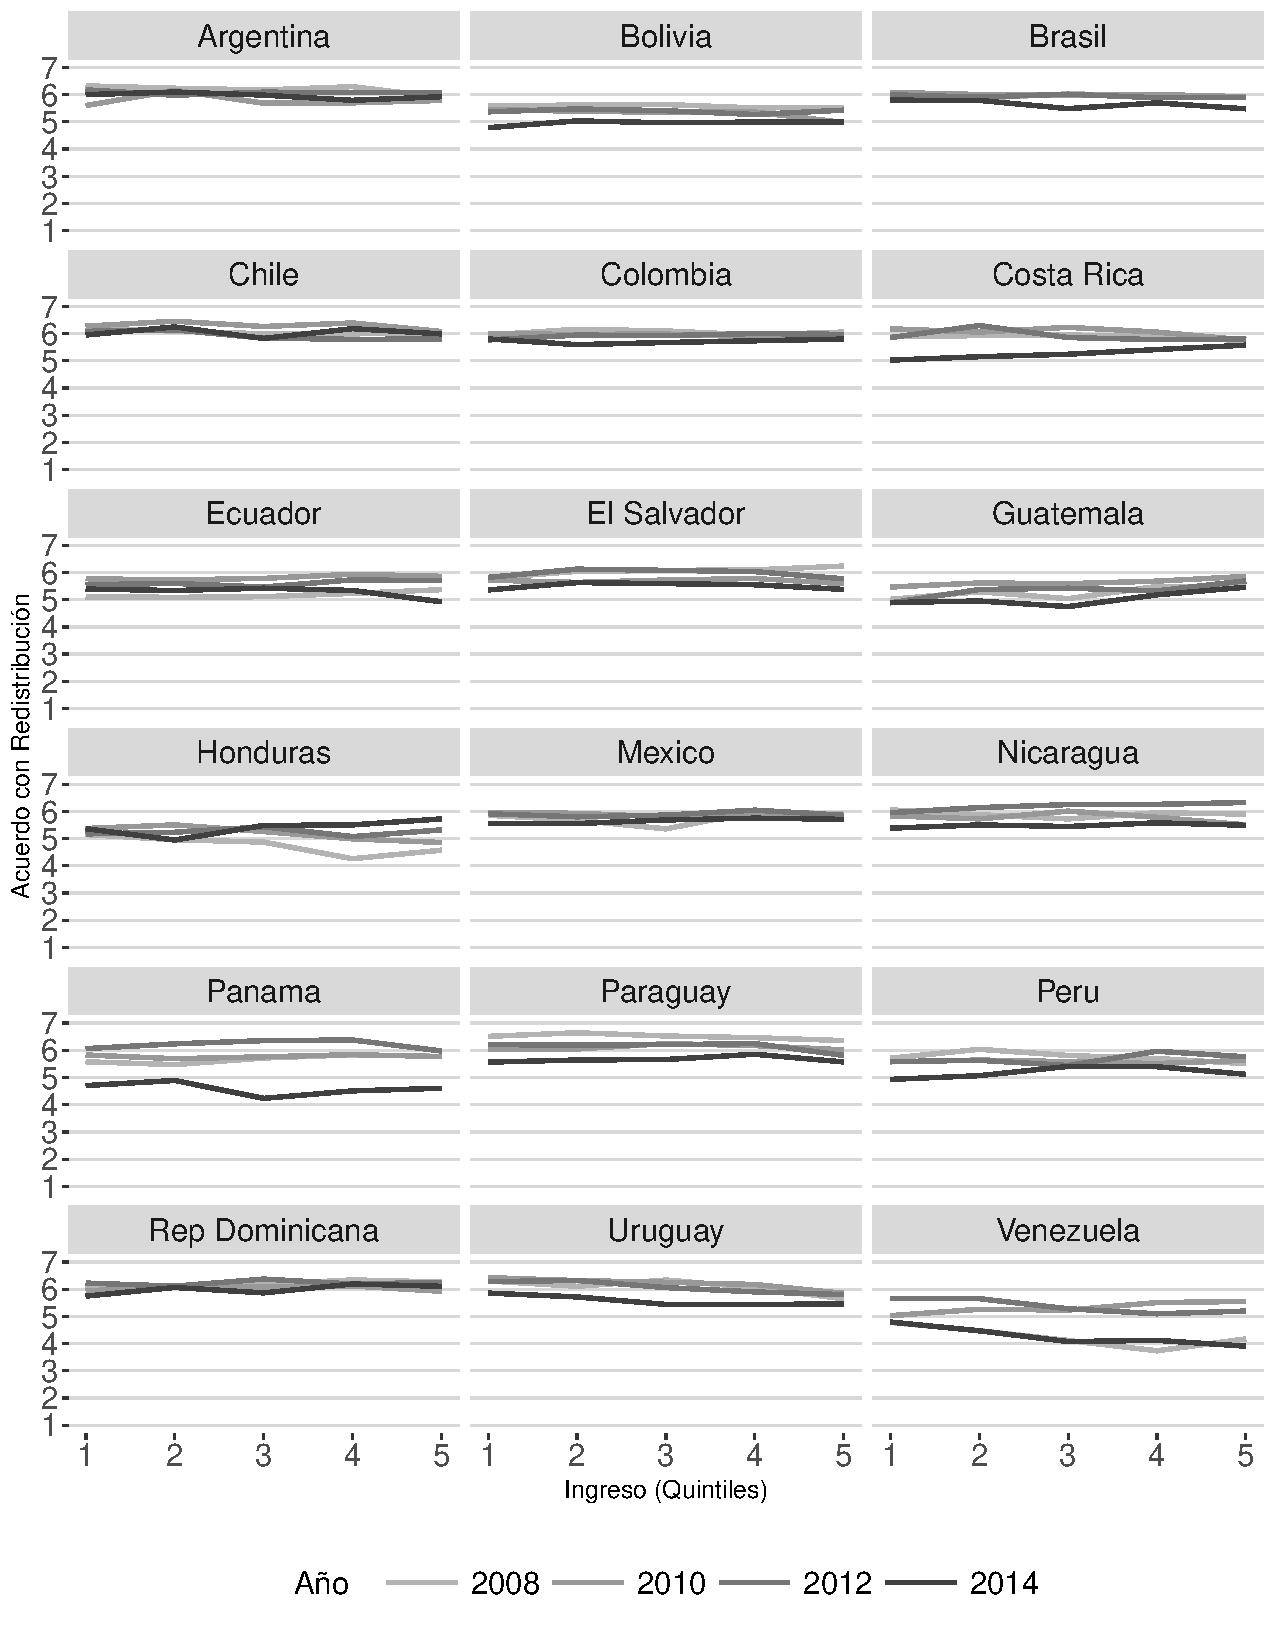
\includegraphics[width=1\textwidth]{G9.pdf}
		\label{fig:g4}
	\end{figure}
\end{center}

\newpage

\subsection{Desigualdad: Relación "entre" países \label{sec:sec62}}

\begin{center}
	\begin{figure}[H]
		\caption[Acuerdo con redistribución y Desigualdad: Relación "entre" países.]{Acuerdo con redistribución y Desigualdad: Relación "entre" países.}
		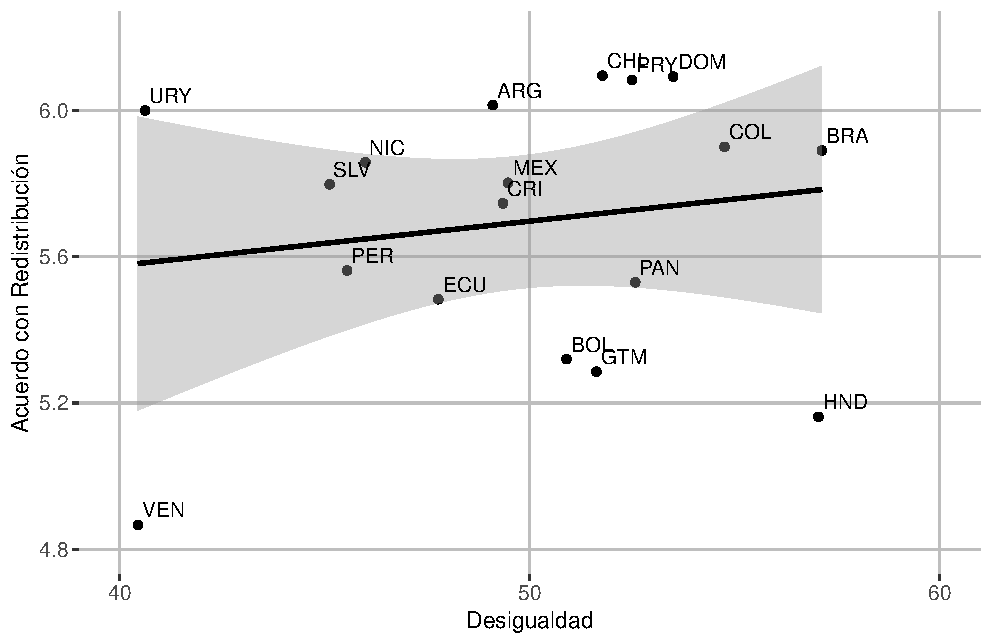
\includegraphics[width=1\textwidth]{G4a.pdf}
		\label{fig:g5}
	\end{figure}
\end{center}

\newpage


\subsection{Desigualdad: Relación "dentro de" países \label{sec:sec63}}

\begin{center}
	\begin{figure}[H]
		\caption[Acuerdo con redistribución y Desigualdad: Relación "dentro de" países.]{Acuerdo con redistribución y Desigualdad: Relación "dentro de" países.}
		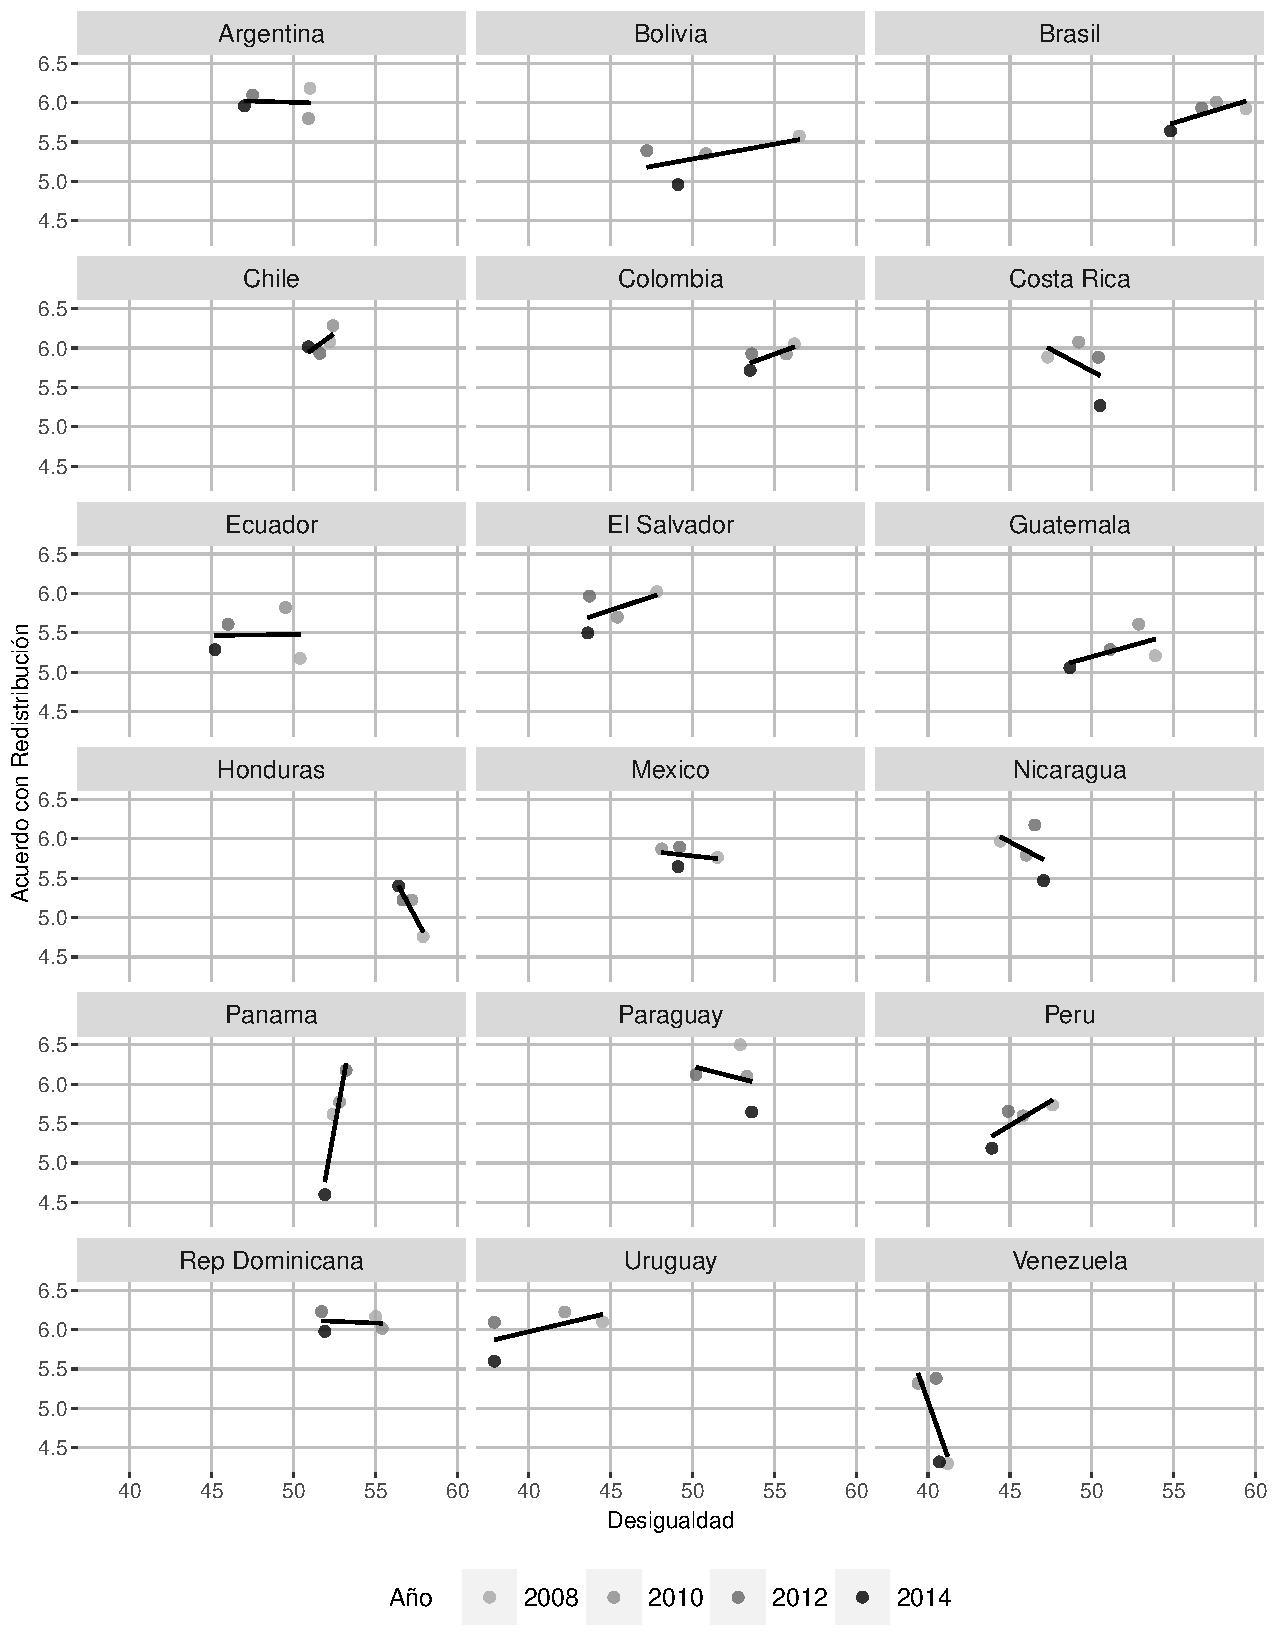
\includegraphics[width=1\textwidth]{G4c.pdf}
		\label{fig:g6}
	\end{figure}
\end{center}

\newpage


\subsection{Desarrollo económico: Relación "entre" países \label{sec:sec64}}

\begin{center}
	\begin{figure}[H]
		\caption[Acuerdo con redistribución y Desarrollo económico: Relación "entre" países]{Acuerdo con redistribución y Desarrollo económico: Relación "entre" países}
		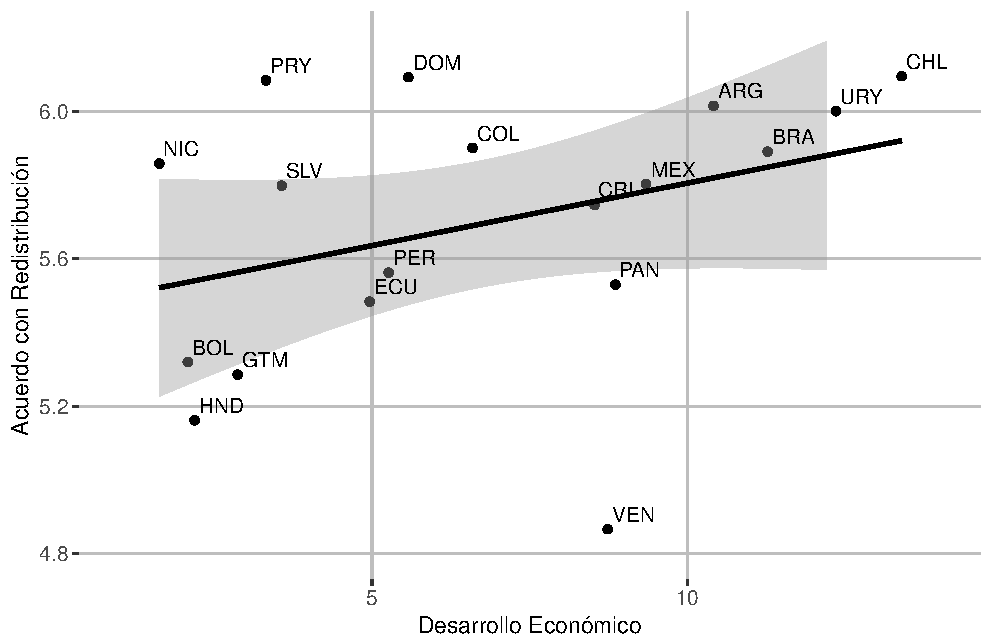
\includegraphics[width=1\textwidth]{G5a.pdf}
		\label{fig:g7}
	\end{figure}
\end{center}

\newpage


\subsection{Desarrollo económico: Relación "dentro de" países \label{sec:sec65}}


\begin{center}
		\begin{figure}[H]
		\caption[Acuerdo con redistribución y Desarrollo económico: Relación "dentro de" países.]{Acuerdo con redistribución y Desarrollo económico: Relación "dentro de" países}
		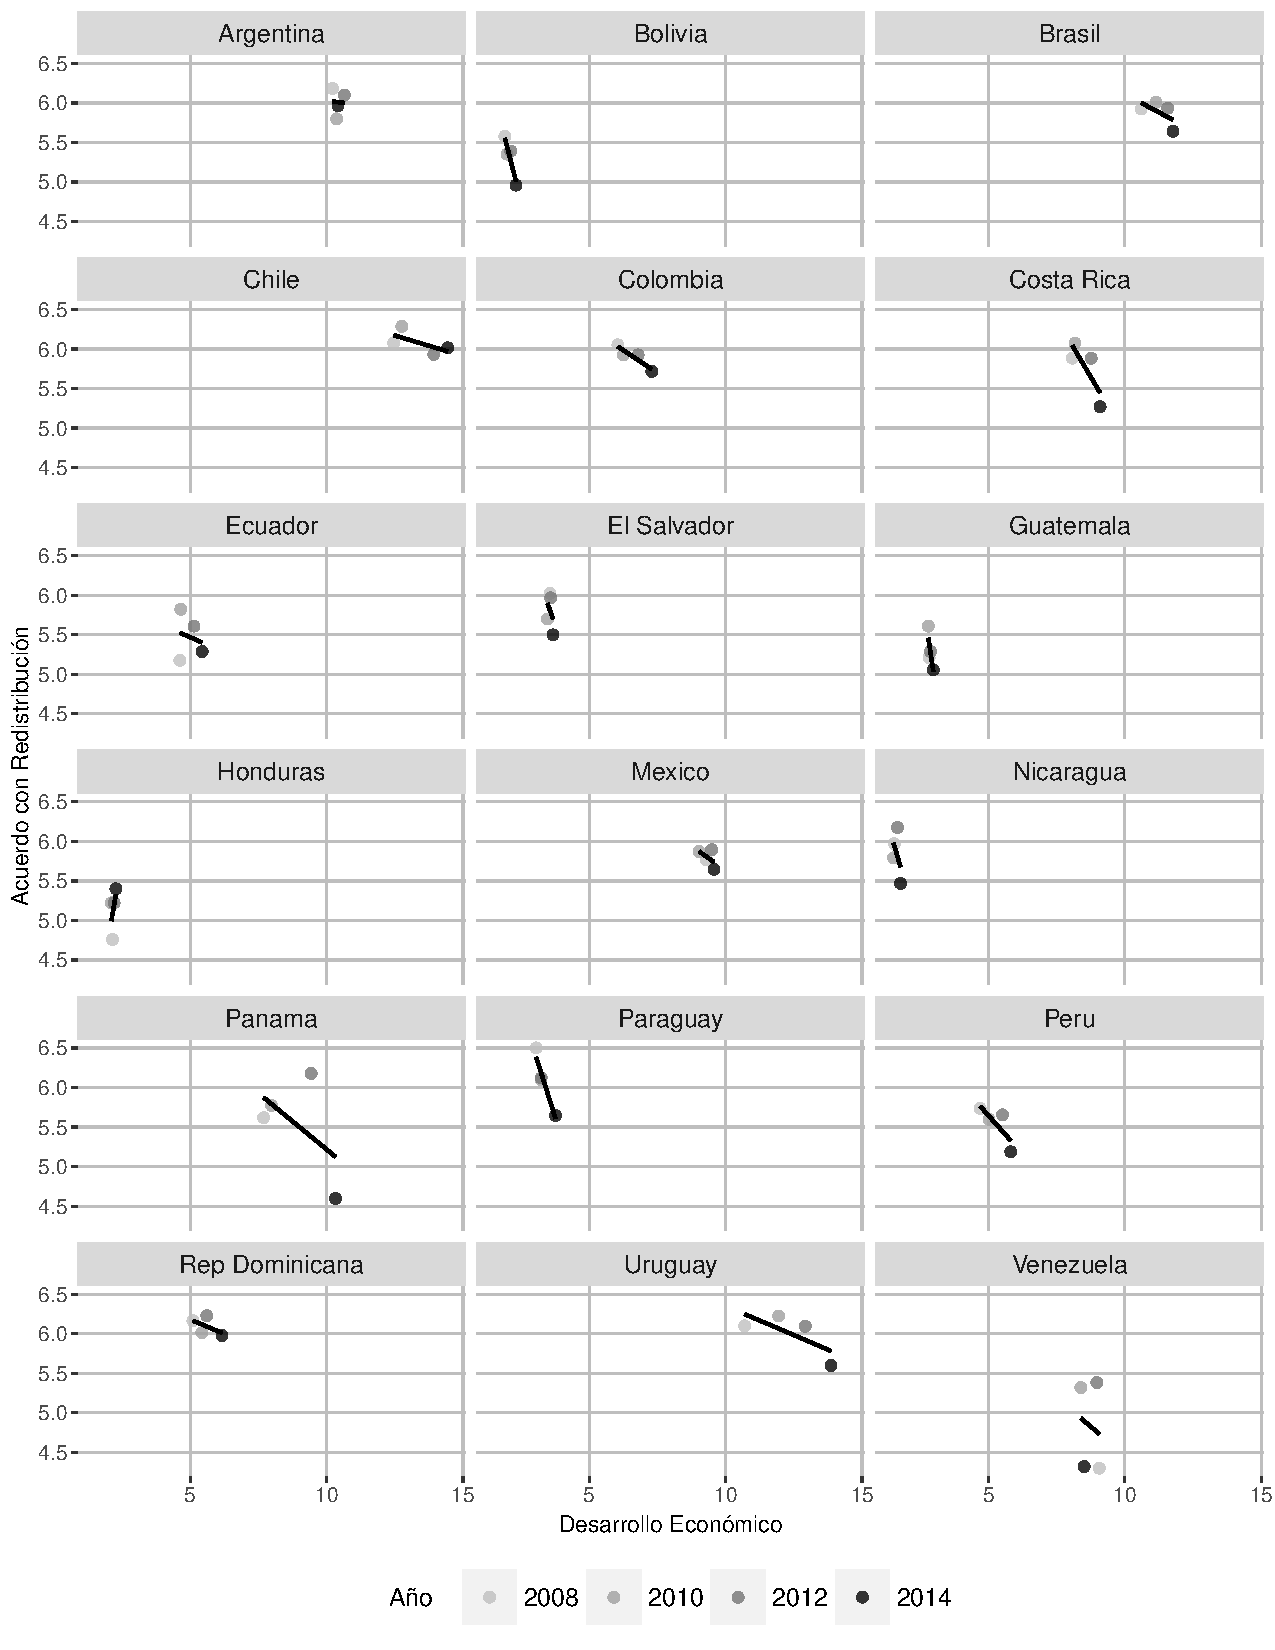
\includegraphics[width=1\textwidth]{G5c.pdf}
		\label{fig:g8}
	\end{figure}
\end{center}

\end{document}
